% !TeX encoding = UTF-8
% !TeX spellcheck = en_US

\documentclass[fontset=mac]{thuthesis}
 
% !TeX root = ./thuthesis-example.tex

% 论文基本信息配置

% 技术方案基本信息配置（简化版）

% 修复 TimesNewRoman 不支持小型大写字母 (small caps) 的警告
% fontspec 加载 Times New Roman 后内部族名为 TimesNewRoman(0)
% 声明 sc 字形回退到 n，消除 NFSS undefined shape 警告
\AtEndPreamble{%
  \DeclareFontShape{TU}{TimesNewRoman(0)}{m}{sc}{<->ssub*TimesNewRoman(0)/m/n}{}%
  \DeclareFontShape{TU}{TimesNewRoman(0)}{bx}{sc}{<->ssub*TimesNewRoman(0)/bx/n}{}%
}

% 载入所需的宏包

% 定理类环境宏包
\usepackage{amsthm}
% 也可以使用 ntheorem
% \usepackage[amsmath,thmmarks,hyperref]{ntheorem}

% 数学字体配置已简化，使用默认设置

% 可以使用 nomencl 生成符号和缩略语说明
% \usepackage{nomencl}
% \makenomenclature

% 表格加脚注
\usepackage{threeparttable}

% 表格中支持跨行
\usepackage{multirow}
\usepackage{ragged2e}

% 固定宽度的表格。
% \usepackage{tabularx}

% 跨页表格
\usepackage{longtable}
\usepackage{tabularx}
\usepackage{booktabs}  % 提供了 \toprule, \midrule, \bottomrule
\newcolumntype{L}[1]{>{\RaggedRight\arraybackslash}p{#1}}
% 算法
\usepackage{algorithm}
\usepackage{algpseudocode}
\usepackage{listings}
\lstset{
  breaklines=true,
  breakatwhitespace=false,
  columns=fullflexible,
  keepspaces=true
}
%代码字体与颜色
\usepackage{xcolor}
\definecolor{deepblue}{rgb}{0,0,0.5}
\definecolor{deepred}{rgb}{0.6,0,0}
\definecolor{deepgreen}{rgb}{0,0.5,0}
\definecolor{codebg}{RGB}{248,248,248}
\definecolor{termblack}{RGB}{40,44,52}
\definecolor{termgray}{RGB}{220,220,220}

% tcolorbox 代码块和终端环境
\usepackage[most,skins]{tcolorbox}
\IfFontExistsTF{Fira Mono}{%
  \setmonofont{Fira Mono}[Scale=0.82]%
}{%
  \IfFontExistsTF{DejaVu Sans Mono}{%
    \setmonofont{DejaVu Sans Mono}[Scale=0.82]%
  }{}%
}

% 量和单位
\usepackage{siunitx}

% 参考文献使用 BibTeX + natbib 宏包
% 顺序编码制
\usepackage[numbers,sort]{natbib}
\bibliographystyle{thuthesis-numeric}
\usepackage{titlesec}

% 让 \paragraph 参与编号（段级别=4）
\setcounter{secnumdepth}{4}

% 定义 \paragraph 的编号样式为纯阿拉伯数字：1, 2, 3, ...
\makeatletter
\renewcommand\theparagraph{\arabic{paragraph}}
% 如果希望每个 section 内从 1 重新开始编号，保留下一行；
% 如果希望全文连续编号，请删掉下一行。
\@addtoreset{paragraph}{section}
\makeatother

% 把 \paragraph 改成块级标题（标题后换行）
\titleformat{\paragraph}[block]
  {\normalfont\normalsize\bfseries}% 样式
  {\theparagraph}%                  % 显示的编号（比如 1, 2, 3）
  {0.8em}%                          % 编号与标题的间距
  {}                                % 标题前置代码

% 调整段前段后间距（可按需修改）
\titlespacing*{\paragraph}
  {0pt}{3.25ex plus 1ex minus .2ex}{1ex plus .2ex}
\usepackage{indentfirst}  % 首行缩进
\usepackage{fancyhdr}

\AtBeginDocument{%
  \pagestyle{fancy}%
  \fancyhf{}%
  \fancyhead[C]{\songti\zihao{-5} 计算机信息工程学院大作业报告}%
  \fancyfoot[C]{\thepage}%
  \renewcommand{\headrulewidth}{0.4pt}%
  \fancypagestyle{plain}{%
    \fancyhf{}%
    \fancyhead[C]{\songti\zihao{-5} 计算机信息工程学院大作业报告}%
    \fancyfoot[C]{\thepage}%
    \renewcommand{\headrulewidth}{0.4pt}%
  }%
  \fancypagestyle{abstractcn}{%
    \fancyhf{}%
    \fancyhead[C]{\songti\zihao{-5} 计算机信息工程学院大作业报告}%
    \renewcommand{\headrulewidth}{0.4pt}%
  }%
  \fancypagestyle{abstracten}{%
    \fancyhf{}%
    \fancyhead[C]{\rmfamily\zihao{-5} Abstract}%
    \renewcommand{\headrulewidth}{0.4pt}%
  }%
}

% 著者-出版年制
% \usepackage{natbib}
% \bibliographystyle{thuthesis-author-year}

% 生命科学学院要求使用 Cell 参考文献格式（2023 年以前使用 author-date 格式）
% \usepackage{natbib}
% \bibliographystyle{cell}

% 本科生参考文献的著录格式
% \usepackage[sort]{natbib}
% \bibliographystyle{thuthesis-bachelor}

% 参考文献使用 BibLaTeX 宏包
% \usepackage[style=thuthesis-numeric]{biblatex}
% \usepackage[style=thuthesis-author-year]{biblatex}
% \usepackage[style=gb7714-2015]{biblatex}
% \usepackage[style=apa]{biblatex}
% \usepackage[style=mla-new]{biblatex}
% 声明 BibLaTeX 的数据库
% \addbibresource{ref/refs.bib}
%可固定下划线长度
\makeatletter
\newcommand\dlmu[2][4cm]{\hskip1pt\underline{\hb@xt@ #1{\hss#2\hss}}\hskip3pt}
\makeatother

\titleformat{\section}[block]{\Large\bfseries}{\thesection}{1em}{}
% 定义所有的图片文件在 figures 子目录下
\graphicspath{{figures/}}

% 数学命令
\makeatletter
\newcommand\dif{%  % 微分符号
  \mathop{}\!%
  \ifthu@math@style@TeX
    d%
  \else
    \mathrm{d}%
  \fi
}
\makeatother

% 代码块环境：浅色背景 + 行号 + 语法高亮
\newtcblisting{codeblock}[2][]{%
  enhanced, breakable,
  listing only,
  colback=codebg, colframe=codebg!60!black,
  fonttitle=\small\sffamily\bfseries,
  title=#2, attach boxed title to top left={yshift=-2mm, xshift=5mm},
  boxed title style={colback=codebg!60!black, size=small},
  left=4mm, right=3mm, top=4mm, bottom=3mm,
  boxrule=0.6pt, arc=2pt,
  listing options={
    language=#1, style=tcblatex,
    basicstyle=\small\ttfamily,
    keywordstyle=\bfseries\color{deepblue},
    stringstyle=\color{deepgreen},
    commentstyle=\itshape\color{gray},
    numbers=left, numberstyle=\tiny\color{gray},
    numbersep=6pt, stepnumber=1,
    showstringspaces=false,
    breaklines=true, breakatwhitespace=false,
    columns=fullflexible, keepspaces=true,
    tabsize=4, xleftmargin=1em
  }
}

% 终端环境：深色背景 + 仿终端样式
\newtcblisting{terminal}[1][]{%
  enhanced, breakable,
  listing only,
  colback=termblack, colframe=termblack,
  fonttitle=\small\ttfamily,
  title={\color{white}$\triangleright$~#1},
  attach boxed title to top left={yshift=-2mm, xshift=5mm},
  boxed title style={colback=termblack!70!white, size=small},
  left=4mm, right=3mm, top=4mm, bottom=3mm,
  boxrule=0.6pt, arc=2pt,
  listing options={
    language=bash, style=tcblatex,
    basicstyle=\small\ttfamily\color{white},
    keywordstyle=\color{cyan!70!white}\bfseries,
    stringstyle=\color{green!60!white},
    commentstyle=\color{gray}\itshape,
    showstringspaces=false,
    breaklines=true, breakatwhitespace=false,
    columns=fullflexible, keepspaces=true,
    tabsize=4
  }
}

% 保留兼容性：旧 \ttb/\ttm 命令（逐步迁移后可删除）
\newcommand{\ttb}{\bfseries\ttfamily}
\newcommand{\ttm}{\ttfamily}

% 保留兼容性：C++ 代码环境
\newcommand\cppstyle{\lstset{
    language=C++,
    basicstyle=\ttfamily,
    morekeywords={self},
    keywordstyle=\bfseries\color{deepblue},
    emph={MyClass,__init__},
    emphstyle=\bfseries\color{deepred},
    stringstyle=\color{deepgreen},
    frame=tb,
    showstringspaces=false,
    captionpos=t
}}
\lstnewenvironment{cpp}[1][]{\cppstyle\lstset{#1}}{}

% hyperref 宏包在最后调用
\usepackage{hyperref}

\begin{document}
\begin{titlepage}
  \newgeometry{top=1.85cm,bottom=2.1cm,left=2.55cm,right=2.55cm}
  \thispagestyle{empty}

  \begin{flushright}
    {\fontsize{14pt}{16pt}\selectfont\fbox{\rule{0pt}{0.78cm}\makebox[2.65cm]{KC021-1}}}
  \end{flushright}

  \vspace{1.05cm}

  \begin{center}
    
\includegraphics[width=7.15cm]{cover/cit-cover-template.jpeg}

    \vspace{1.12cm}

    {\rmfamily\fontsize{16pt}{20pt}\selectfont
      CHANGZHOU\quad INSTITUTE\quad OF\quad TECHNOLOGY\par}

    \vspace{1.55cm}

    {\heiti\bfseries\fontsize{30pt}{36pt}\selectfont 课程大作业说明书\par}
  \end{center}

  \vspace{1.35cm}

  \begingroup
  \setlength{\parindent}{0pt}
  \fontsize{18pt}{24pt}\selectfont
  \newcommand{\coverlabel}[1]{\makebox[3.55cm][l]{\heiti\bfseries #1}}
  \newcommand{\coverlabelfour}[1]{\coverlabel{\makebox[4em][l]{#1}：}}
  \newcommand{\coverline}[1]{\underline{\makebox[7.9cm][c]{#1}}}
  \begin{center}
    \begin{minipage}{11.8cm}
      \coverlabelfour{课程名}\coverline{分布式应用开发技术（Q）}\par\vspace{0.62cm}
      \coverlabelfour{题目}\coverline{\fontsize{15pt}{24pt}\selectfont \shortstack[c]{面向社交图谱与消息投递的\\分布式推荐系统}}\par\vspace{1.08cm}
      \coverlabelfour{二级学院}\coverline{计算机信息工程学院}\par\vspace{0.3cm}
      \coverlabelfour{专业}\coverline{软件工程}\par\vspace{0.3cm}
      \coverlabelfour{班级}\coverline{23软一}\par\vspace{0.3cm}
      \coverlabelfour{学号姓名}\coverline{23030327\quad 许子祺}\par\vspace{0.3cm}
      \hspace*{3.55cm}\coverline{23030315\quad 莫文涛}\par\vspace{0.3cm}
      \hspace*{3.55cm}\coverline{23030316\quad 钱季清}\par\vspace{0.3cm}
      \hspace*{3.55cm}\coverline{23250123\quad 王奕泽}\par\vspace{0.3cm}
      \coverlabelfour{指导教师}\coverline{江亮}\par
    \end{minipage}
  \end{center}
  \endgroup

  \vfill

  \begin{center}
    {\songti\fontsize{16pt}{20pt}\selectfont 2026 年 6 月\par}
  \end{center}
  \restoregeometry
\end{titlepage}


\frontmatter
% !TeX root = ../thuthesis-example.tex

% 中英文摘要和关键字
\clearpage
\thispagestyle{abstractcn}
\addcontentsline{toc}{chapter}{摘 要}

\vspace*{1.15cm}

\begin{center}
  {\heiti\bfseries\zihao{2} 基于Spring Boot的分布式推荐系统\par}
  \vspace{0.55cm}
  {\heiti\bfseries\zihao{3} 摘\quad 要\par}
\end{center}

\vspace{0.25cm}

{\songti\zihao{-4}\setlength{\parindent}{2em}\linespread{1.65}\selectfont
本文围绕“基于Spring Boot的分布式推荐系统”展开设计与实现说明。系统面向类即时通信与内容社区场景，在保留前端交互、新闻内容、用户关系与推荐算法思想的基础上，将后端设计为Spring Boot分层服务。系统通过RESTful接口接收前端请求，利用Supabase PostgreSQL保存用户、群组、联系人、新闻内容、用户行为、用户兴趣向量与实验配置等数据，并结合Redis完成时间线缓存、热点Feed缓存和临时特征缓存。

推荐模块是本项目的核心。系统采用“请求上下文构建、特征补全、多路召回、候选补全、规则过滤、加权评分、TopK选择、曝光记录”的流水线结构。召回阶段综合关注关系、社交图谱、新闻向量、作者兴趣、热门内容与冷启动内容；过滤阶段处理去重、已曝光内容、自身内容、屏蔽关系和敏感词；排序阶段使用行为权重、作者亲和度、内容质量、新鲜度和校准因子进行融合评分。该设计既保证推荐结果具备个性化，又兼顾系统吞吐量、可解释性和可灰度发布能力。

系统采用Apifox进行接口联调，围绕推荐Feed接口、趋势接口、用户推荐接口和行为埋点接口设计测试用例。通过Supabase MCP读取云端数据库结构后，本文给出了数据库实体关系和关键表字段说明。测试结果表明，该方案能够支撑课程要求中的分布式后端、云端数据库、前后端分离、接口联调与推荐算法设计等核心内容，具备继续扩展为真实线上服务的工程基础。

\vspace{0.65cm}
\noindent{\heiti 关键词：}Spring Boot；分布式系统；推荐算法；Supabase；Apifox
\par}

\clearpage
\thispagestyle{abstracten}
\addcontentsline{toc}{chapter}{Abstract}

\vspace*{0.9cm}

\begin{center}
  {\rmfamily\bfseries\zihao{3} Spring Boot Based Distributed Recommendation System\par}
  \vspace{0.45cm}
  {\rmfamily\bfseries\zihao{3} Abstract\par}
\end{center}

\vspace{0.15cm}

{\rmfamily\zihao{-4}\setlength{\parindent}{2em}\linespread{1.45}\selectfont
This report presents the design of a distributed recommendation system based on Spring Boot. The system targets an instant-messaging and content-community scenario. While preserving the existing front-end interaction, news content, user relationship, and recommendation ideas, the back-end is redesigned as a layered Spring Boot service. The system exposes RESTful APIs, stores users, groups, contacts, news articles, user events, user vectors, and experiment configurations in Supabase PostgreSQL, and uses Redis for timeline cache, hot feed cache, and temporary feature cache.

The recommendation module is the core of the project. It follows a pipeline consisting of request context construction, feature hydration, multi-source recall, candidate hydration, rule-based filtering, weighted scoring, TopK selection, and impression logging. The recall stage combines following timelines, social graph expansion, news vector retrieval, author-interest matching, popular content, and cold-start content. The filtering stage removes duplicates, seen items, self-authored items, blocked users, and sensitive keywords. The ranking stage fuses behavior weights, author affinity, content quality, recency, and calibration factors. This design balances personalization, throughput, interpretability, and gradual rollout capability.

Apifox is used for API integration testing, covering the recommendation feed API, trend API, user recommendation API, and behavior tracking API. Based on the Supabase MCP inspection, this report documents the cloud database schema and key entity relationships. The project satisfies the course requirements for a distributed back-end, cloud database, front-end/back-end separation, API testing, and recommendation algorithm design.

\vspace{0.45cm}
\noindent{\bfseries Keywords:} Spring Boot; Distributed System; Recommendation Algorithm; Supabase; Apifox
\par}


% 目录
\tableofcontents

% 插图和附表清单
% \listoffiguresandtables  % 插图和附表清单

% 正文部分
\mainmatter
% !TeX root = ../thuthesis-example.tex

\chapter{引言}

\section{项目目的}

随着移动互联网应用的发展，用户每天接触到的消息、新闻、群组动态和社交内容不断增加。传统按时间倒序展示内容的方式实现简单，但在内容数量较大时容易出现两个问题：一是用户真正关心的内容被大量低相关内容淹没；二是系统无法根据用户兴趣、关注关系和近期行为动态调整内容排序。推荐系统的引入可以在“内容生产者”和“内容消费者”之间建立更有效的匹配关系，使用户在较短时间内看到更有价值的内容。

本项目以类Telegram社交应用为业务背景，设计一套基于Spring Boot的分布式推荐系统。项目目标不是单纯完成一个接口，而是从课程设计角度形成完整的工程闭环：前端负责页面展示和交互，Spring Boot后端负责接口、业务编排、推荐算法与安全控制，Supabase PostgreSQL负责云端持久化数据，Redis负责缓存和时间线加速，Apifox负责接口联调和测试记录。

本项目重点解决以下问题：

\begin{enumerate}
  \item 构建符合分布式应用课程要求的后端架构。后端采用Spring Boot进行模块划分，按控制层、服务层、仓储层和算法策略层组织代码，避免把接口、业务逻辑和数据访问混在同一个文件中。
  \item 建立真实可解释的推荐算法流程。推荐系统不是只按浏览量排序，而是综合用户关注关系、内容标签、行为事件、兴趣向量、热点内容、冷启动策略和实验配置进行候选生成与排序。
  \item 接入云端数据库。系统使用Supabase PostgreSQL保存用户、群组、联系人、新闻内容、用户行为、兴趣向量和实验配置，使数据结构具备远程访问、持久化和后续扩展能力。
  \item 完成接口联调与测试。通过Apifox构造推荐Feed接口请求，验证请求参数、接口路径和返回结构，为后续自动化测试和接口文档共享打基础。
\end{enumerate}

从工程角度看，本项目将推荐逻辑拆分为多个阶段，每个阶段只承担清晰的职责：召回阶段负责扩大候选集，过滤阶段负责保证候选安全和有效，评分阶段负责计算相关性，选择阶段负责控制数量和多样性，副作用阶段负责记录曝光与实验数据。这种分层流水线思想有利于后续替换算法、扩展数据源和定位问题。

\section{本文组织结构}

本文按照课程大作业报告模板组织内容，章节安排如下：

第一章为引言，说明项目背景、项目目的和报告组织结构。

第二章为相关技术概述，介绍Spring Boot、Spring Cloud思想、Supabase PostgreSQL、Redis、Apifox、React前端以及个性化推荐算法等关键技术。

第三章为系统分析设计，围绕需求分析、可行性分析、系统架构、模块设计、数据库设计和推荐算法设计展开说明，并给出系统架构图、推荐算法流程图和数据库实体关系图。

第四章为项目测试，说明接口测试环境、Apifox联调过程、核心接口测试方案、数据库检查结果以及测试中发现的安全风险。

第五章为总结与展望，总结本项目完成的主要工作，分析目前仍然存在的不足，并提出后续在微服务拆分、模型训练、安全策略和监控运维方面的改进方向。

% !TeX root = ../thuthesis-example.tex

\chapter{相关技术概述}

\section{Spring Boot后端开发技术}

Spring Boot是Java生态中常用的后端开发框架，它通过自动配置、起步依赖和内嵌Web容器降低了服务搭建成本。对于本项目而言，Spring Boot主要承担REST接口、业务编排、数据访问、鉴权拦截和推荐算法调度等职责。系统可按照Controller、Service、Repository、Domain、Config等层次组织代码，使接口入口、业务规则和数据库访问边界清晰。

在推荐系统场景中，Spring Boot的优势体现在三个方面。第一，接口层可以使用\texttt{@RestController}和\texttt{@RequestMapping}快速定义推荐Feed、趋势内容、用户推荐和行为埋点接口。第二，服务层可以通过依赖注入组合多个召回源、过滤器和评分器，便于替换算法策略。第三，配合Spring Security和JWT可以对用户身份进行校验，避免推荐接口在未授权情况下暴露用户画像和行为数据。

\section{Spring Cloud与分布式思想}

本项目虽然以课程设计为主，但后端设计遵循Spring Cloud的分布式思想。推荐系统可以拆分为用户服务、群组服务、内容服务、推荐服务、实验服务和日志服务。实际部署时，这些服务既可以先以单体Spring Boot应用中的多模块方式实现，也可以在业务增长后逐步拆分为微服务。

在分布式系统中，推荐服务需要关注调用链稳定性和缓存策略。用户画像、关注关系和内容特征来自不同数据源，若每次请求都同步查询全部数据，会导致接口响应变慢。因此系统将部分热点数据放入Redis缓存，并对召回源设置超时时间。当某一路召回失败时，系统可以回退到热门内容或冷启动内容，保证Feed接口可用。

\section{Supabase PostgreSQL云端数据库}

Supabase是基于PostgreSQL的后端即服务平台，提供托管数据库、认证、存储和实时能力。本项目使用Supabase作为云端数据库，项目名称为\texttt{telegram}，区域为\texttt{us-west-2}，数据库版本为PostgreSQL 17。通过MCP读取可知，数据库中已经存在用户、群组、联系人、新闻内容、用户行为、用户兴趣向量和实验配置等表。

相比本地数据库，Supabase的优势是部署简单、云端访问方便、适合课程设计展示。对于推荐系统而言，\texttt{news\_articles}表保存内容特征，\texttt{news\_user\_events}表保存点击、停留和分享等行为，\texttt{news\_user\_vectors}表保存短期和长期兴趣向量，\texttt{experiments}表保存实验分桶策略。这些表共同支撑个性化推荐的输入数据。

\section{Redis缓存技术}

Redis是内存型键值数据库，常用于缓存、排行榜、计数器和分布式锁。本项目在推荐系统中使用Redis承担三个职责：

\begin{enumerate}
  \item 时间线缓存。将作者最新内容写入有序集合，例如按作者维护最近七天内容，用户请求时按关注列表聚合候选内容。
  \item 热点内容缓存。将高点击、高分享和高互动内容缓存为热门候选，作为冷启动和召回失败时的兜底来源。
  \item 临时特征缓存。缓存用户近期行为、已曝光内容和请求追踪标识，减少数据库重复查询。
\end{enumerate}

Redis缓存不替代数据库持久化，而是作为提高吞吐量和降低延迟的中间层。推荐接口每次请求都可能触发多路召回和特征补全，缓存可以显著减少数据库压力。

\section{Go消息投递与Redis Stream消费技术}

Go语言具有轻量级协程、通道和高效网络库，适合实现高并发消息消费、异步投递和后台任务执行。本项目在Spring Boot业务服务之外，引入Go侧消息投递服务，主要处理平台事件、消息投递、同步唤醒和outbox状态更新。该服务不直接替代业务后端，而是承担高频、异步、可恢复的投递链路，使主业务接口可以将耗时的多接收者分发工作转移到后台执行。

Go投递服务的核心输入来自Redis Stream。Redis Stream支持消费者组、消息确认、待处理消息列表（PEL）和消息重放，适合表达“至少一次投递”和失败恢复语义。为了避免全局串行消费带来的吞吐瓶颈，Go侧按照\texttt{chat\_id}优先、其次\texttt{user\_id}、\texttt{outbox\_id}或\texttt{message\_id}的方式计算消息分区键，将消息派发到多个worker lane。同一业务键在同一lane内保持顺序，不同业务键可以并行处理，从而兼顾即时通信系统中的顺序要求和大群消息扇出的并发需求。

在确认机制上，服务将成功消息按stream聚合后批量\texttt{XACK}，减少Redis远程往返；失败消息仍保留原有重试、恢复和死信语义。对于PEL reclaim，系统将其从主消费循环中拆分为独立的有预算后台worker，避免旧消息恢复阻塞新消息读取。为了降低MongoDB写放大，投递链路还引入分块update id预留、outbox聚合状态增量维护和批量wake事件发布。上述设计体现了分布式消息系统中常见的三个原则：顺序只在必要的业务键内保证、远程操作尽量批处理、恢复逻辑不阻塞主路径。

\section{C++图计算与快照查询技术}

C++适合实现对延迟和内存布局敏感的图查询内核。本项目在推荐召回阶段需要频繁查询用户的邻居关系、共同联系人、共同群组和多跳社交路径。如果所有图关系都在通用业务服务中逐条查询数据库，会造成较高的远程访问成本和不可控的尾延迟。因此系统引入C++图计算服务，将社交图谱预构建为内存快照，通过HTTP接口向推荐服务提供高性能图查询能力。

图计算服务采用快照发布模型。后端服务负责提供图快照数据，C++服务定期从\texttt{/internal/graph-kernel/snapshot}拉取并构建内存索引。快照构建阶段将用户id和边类型intern为整数编号，再按源点组织为紧凑CSR（Compressed Sparse Row）结构。CSR结构使用连续数组保存邻居和offset，相比散列表或对象数组可以减少内存碎片，提高缓存命中率，也便于对高出度节点执行顺序扫描和TopK截断。

在查询层，C++服务支持直接邻居查询、ranked邻居查询、overlap共同关系查询和多跳遍历。为了控制高出度节点带来的开销，系统将请求级时间\texttt{now\_ms}采样一次，并在ranking和traversal中复用同一个时间基准，避免热循环重复系统调用。overlap查询采用streaming top-K思想，不必先物化全部交集再排序，而是在扫描过程中维护候选上限。多跳遍历采用budget-aware策略，在访问预算内优先保留更有价值的候选。服务还为快照版本、快照表示、构建阶段耗时、扫描数、访问数和预算耗尽情况输出summary和metrics，方便推荐服务判断图召回是否健康。

\section{Apifox接口联调技术}

Apifox是一体化API协作工具，支持接口设计、请求调试、接口文档和自动化测试。本项目使用Apifox对Spring Boot后端接口进行联调。测试时可以在请求栏中输入本地服务地址，例如\texttt{http://localhost:8080/api/space/feed}，并通过Params区域配置\texttt{limit}、\texttt{in\_network\_only}等参数。

在课程报告中，Apifox截图不仅用于展示测试工具，也用于证明接口路径、请求方法、参数拆解和联调过程。后续如果接入真实Spring Boot运行服务，还可以在Apifox中保存接口集合，设置环境变量、Authorization请求头和响应断言。

\section{前端React与TypeScript技术}

系统前端采用React与TypeScript思想进行设计。React负责组件化页面展示，TypeScript为接口数据结构提供类型约束。前端主要页面包括用户登录、群组与联系人、新闻列表、推荐Feed、趋势内容、用户推荐和行为反馈。前端向后端发送HTTP请求，后端返回JSON格式数据，前端再根据返回的内容渲染列表、卡片和交互按钮。

在推荐系统中，前端不仅展示推荐结果，也承担行为采集入口。例如用户点击新闻、停留阅读、分享内容或屏蔽某条内容时，前端可以向后端行为埋点接口上报事件。后端将事件写入\texttt{news\_user\_events}，推荐服务再根据这些行为更新兴趣向量和排序权重。

\section{个性化推荐算法技术}

个性化推荐算法的核心任务是从大量候选内容中选出最适合当前用户的一组内容。本项目采用多阶段推荐架构，主要包括召回、过滤、排序和重排四个阶段。

召回阶段负责扩大候选集。系统可以从关注作者内容、社交图谱扩展内容、新闻向量近邻、作者兴趣匹配、热门内容和冷启动内容中分别取出候选。不同召回源适合不同用户状态：新用户更依赖热门内容和冷启动策略，活跃用户更适合使用兴趣向量和历史行为，关注关系较丰富的用户则适合使用社交图谱。

过滤阶段负责保证候选内容可用。系统会去除重复内容、用户自己发布的内容、已经曝光过的内容、来自屏蔽用户的内容以及命中敏感词的内容。过滤阶段强调规则确定性，优先保证安全和体验。

排序阶段负责计算候选内容得分。本项目采用加权融合思想，核心特征包括点击、回复、转发、分享、停留时长、作者亲和度、内容质量、新鲜度和负反馈。正向行为提升得分，负向行为降低得分。例如回复和转发代表较强互动意愿，权重高于普通点击；屏蔽、举报和“不感兴趣”属于强负反馈，需要显著降低相关内容排序。

重排阶段负责控制最终结果的多样性。TopK选择不能只选最高分内容，否则可能出现同一作者、同一主题或同一来源连续占据列表的情况。系统在选择阶段加入作者多样性、主题多样性和内容形态约束，使推荐结果更加均衡。

% !TeX root = ../thuthesis-example.tex

\chapter{系统分析设计}

\section{需求分析}

\subsection{功能需求}

本项目面向类即时通信与内容社区系统，核心功能需求如下：

\begin{enumerate}
  \item 用户与关系管理。系统需要支持用户资料、联系人关系、关注关系、群组成员关系等数据管理，为推荐系统提供社交图谱基础。
  \item 内容管理。系统需要保存新闻内容、来源、分类、关键词、向量特征、发布时间和互动计数，作为推荐候选内容池。
  \item 推荐Feed生成。系统需要根据用户身份、请求参数、语言、地区、历史曝光和行为特征生成个性化Feed。
  \item 行为埋点。系统需要记录曝光、点击、停留、分享等事件，并将其写入云端数据库，用于后续兴趣更新和算法评估。
  \item 实验配置。系统需要支持不同推荐策略的灰度实验，通过实验配置控制流量比例、分桶方式和评价指标。
  \item 接口联调。系统需要通过Apifox完成关键接口的请求配置、参数检查和测试记录。
\end{enumerate}

\subsection{非功能需求}

除功能需求外，系统还应满足以下非功能需求：

\begin{enumerate}
  \item 可扩展性。推荐召回源、过滤器和评分器应支持独立扩展，避免算法调整影响全部后端逻辑。
  \item 低延迟。Feed接口属于高频接口，应通过缓存、超时控制和候选数量限制降低响应时间。
  \item 可解释性。每条推荐结果应尽量能够追踪其召回来源、主要评分因素和实验分桶。
  \item 安全性。涉及用户资料、密码字段和行为数据的表必须加强访问控制，避免匿名访问造成数据泄露。
  \item 可测试性。接口路径、请求参数和响应结构应能在Apifox中清晰表达，便于课程验收和后续自动化测试。
\end{enumerate}

\section{可行性分析}

\subsection{技术可行性}

Spring Boot提供成熟的Web开发、依赖注入、数据访问和安全控制能力，能够满足后端服务搭建需求。Supabase PostgreSQL已经具备项目所需的核心表结构，能够保存用户、内容、行为和实验数据。Redis适合处理时间线缓存和热点Feed缓存，能够降低数据库压力。Apifox可以完成接口联调和截图取证。因此，从技术栈角度看，本项目具备实现可行性。

\subsection{经济可行性}

项目采用开源框架和云端免费层服务完成课程设计。Spring Boot、React、Redis客户端和大部分推荐算法逻辑均可免费使用。Supabase项目当前处于免费计划，能够满足课程阶段的数据规模。Apifox桌面端可用于本地联调，不需要额外购买商业服务。

\subsection{操作可行性}

系统采用前后端分离方式，用户通过前端页面访问推荐内容，开发者通过Apifox测试接口，管理员可通过Supabase控制台查看数据库。对于课程展示而言，操作路径清晰，既可以展示数据库表结构，也可以展示接口请求配置和推荐算法流程。

\section{项目系统架构}

系统总体架构如图\ref{fig:system_architecture_springboot}所示。整体分为客户端层、业务服务层、异步投递层、图计算层、数据与缓存层、推荐算法层六部分。客户端层包括React前端和Apifox接口联调工具；业务服务层以Spring Boot为核心，负责REST接口、认证与权限、推荐Feed服务、用户与群组服务、新闻内容服务；异步投递层由Go服务负责Redis Stream消费、消息扇出、outbox状态维护和同步唤醒；图计算层由C++服务负责社交图谱快照、邻居查询、共同关系查询和多跳遍历；数据与缓存层包括Redis、Supabase PostgreSQL、MongoDB和对象存储；推荐算法层负责多路召回、过滤规则、加权评分、TopK排序和埋点实验。

\begin{figure}[htbp]
  \centering
  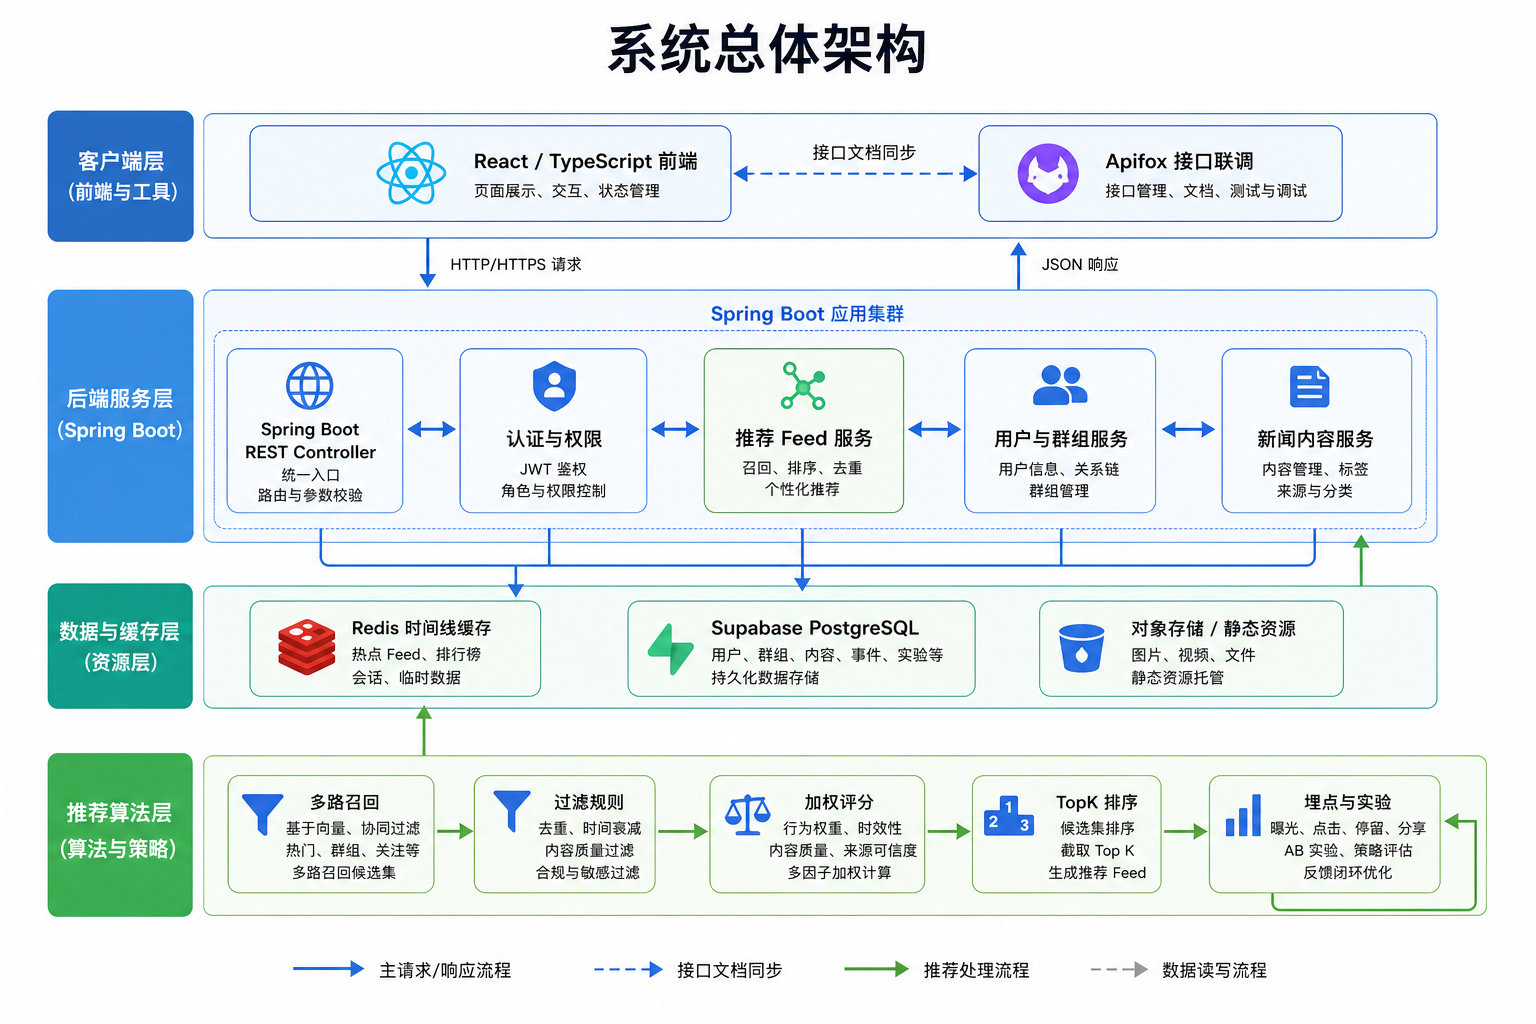
\includegraphics[width=0.95\textwidth]{system-architecture-springboot.png}
  \caption{系统总体架构图}
  \label{fig:system_architecture_springboot}
\end{figure}

后端入口采用REST API。推荐Feed接口可以设计为：

\begin{lstlisting}[language=Java,caption={推荐Feed接口设计示例}]
@RestController
@RequestMapping("/api/space")
public class SpaceFeedController {
    private final RecommendationService recommendationService;

    @GetMapping("/feed")
    public FeedResponse feed(
            @AuthenticationPrincipal LoginUser user,
            @RequestParam(defaultValue = "20") int limit,
            @RequestParam(required = false) String cursor,
            @RequestParam(defaultValue = "false") boolean inNetworkOnly) {
        FeedRequest request = FeedRequest.of(user.getId(), limit, cursor, inNetworkOnly);
        return recommendationService.recommend(request);
    }
}
\end{lstlisting}

该接口将参数解析与业务处理分离。Controller只负责接收请求和校验参数，具体推荐流程交给\texttt{RecommendationService}完成。

\section{项目设计}

\subsection{功能模块设计}

系统按照职责划分为以下模块：

\begin{longtable}{p{0.22\textwidth}p{0.7\textwidth}}
\caption{系统功能模块设计}\\
\toprule
模块 & 主要职责 \\
\midrule
\endfirsthead
\toprule
模块 & 主要职责 \\
\midrule
\endhead
用户模块 & 管理用户资料、登录态、地区、语言、在线状态，为推荐服务提供用户基础画像。\\
关系模块 & 管理联系人、关注关系、群组成员关系，为社交召回和作者亲和度计算提供依据。\\
内容模块 & 管理新闻内容、分类、关键词、向量、发布时间、来源和互动计数。\\
推荐模块 & 编排特征补全、多路召回、候选补全、过滤、评分、TopK选择和曝光记录。\\
Go投递模块 & 消费Redis Stream中的平台事件和消息事件，按业务键并行投递，维护outbox聚合状态，批量ACK并处理失败恢复。\\
C++图计算模块 & 加载社交图谱快照，提供直接邻居、共同关系、ranked邻居和多跳遍历查询，为推荐召回提供低延迟图特征。\\
实验模块 & 维护实验配置、流量比例、实验分桶和评价指标，支持推荐策略灰度发布。\\
测试模块 & 通过Apifox维护接口请求、参数、返回结构和联调截图。\\
\bottomrule
\end{longtable}

\subsection{Go消息投递链路设计}

即时通信系统中的消息投递具有明显的分布式特征：同一会话内的消息需要保持顺序，不同会话之间又需要尽可能并行；投递过程中可能出现Redis读取失败、MongoDB写入超时、接收者状态变化和消费者重启等情况。因此，本项目将投递链路从业务接口中拆分出来，由Go服务独立负责。

Go投递链路的数据流如下：

\begin{enumerate}
  \item Spring Boot业务服务或平台事件总线将消息事件写入Redis Stream。
  \item Go消费者按consumer group读取消息，先解析事件类型和业务分区键。
  \item 调度器根据\texttt{chat\_id}、\texttt{user\_id}、\texttt{outbox\_id}或\texttt{message\_id}选择worker lane。
  \item worker在lane内串行处理同一业务键，执行接收者投影、update id预留、outbox chunk更新和wake事件发布。
  \item 成功消息按stream聚合后批量\texttt{XACK}，失败消息进入重试或死信处理。
\end{enumerate}

该设计的关键是“局部有序、全局并行”。设消息集合为$\mathcal{M}$，业务分区函数为$k(m)$，worker lane数量为$W$，则消息$m$被映射到：

\[
lane(m)=hash(k(m)) \bmod W
\]

对于任意两条消息$m_i,m_j$，若$k(m_i)=k(m_j)$，则二者进入同一lane并按读取顺序处理；若$k(m_i)\ne k(m_j)$，则可以进入不同lane并行处理。这样既不会破坏同一聊天或同一outbox内部的顺序，也避免所有消息被单线程消费限制吞吐。

在写入侧，Go服务使用分块预留降低MongoDB远程写放大。传统做法可能为每个接收者单独申请一个update id，若一个群消息有$n$个接收者，则远程写次数接近$O(n)$。分块预留将多个接收者合并为block，一次远程操作申请连续区间，再在本地分配给接收者，使远程预留次数近似降为$O(\lceil n/B \rceil)$，其中$B$为block大小。outbox状态也不再每次读回所有chunk重算，而是通过增量计数维护\texttt{queuedChunkCount}、\texttt{completedChunkCount}和\texttt{failedChunkCount}，再保留低频reconcile路径用于修复异常状态。

为了支持运维和课程验收，Go服务在summary中记录worker lane数量、ack batch size、batch ack count、reservation mode、wake publish mode、outbox aggregate mode、Mongo失败分类和主投递成功率等字段。通过这些字段可以判断投递链路是否处于高并发模式、是否发生批量ACK、是否出现大量可重试失败，以及是否需要调整worker数量或批量大小。

\subsection{C++图计算内核设计}

推荐系统中的社交召回依赖图结构。用户、联系人、群组、作者和互动关系可以抽象为图$G=(V,E)$，其中$V$表示用户或实体节点，$E$表示关注、联系人、共同群组、互动等边。若在每次推荐请求中动态查询数据库计算共同关系，延迟会受到网络往返和数据库负载影响。C++图计算内核通过内存快照方式，将高频图查询从业务数据库路径中分离出来。

图快照构建分为三个阶段。第一阶段从后端快照接口按页读取边数据，避免一次性加载全部边造成内存峰值。第二阶段将字符串形式的\texttt{source\_user\_id}、\texttt{target\_user\_id}和边类型intern为\texttt{uint32}编号。第三阶段按源点聚合并构建CSR索引：

\[
neighbors(src)=N[offset[src]\,..\,offset[src+1])
\]

其中$offset$数组记录每个源点邻居区间的起止位置，$N$数组连续保存邻居编号、边权和时间信息。该结构适合直接邻居读取和ranked top-K读取，也便于在overlap查询中顺序扫描两个邻居列表。

共同关系查询可表示为两个邻居集合的交集：

\[
overlap(u,v)=N(u)\cap N(v)
\]

如果先物化全部交集再排序，在高出度节点上会消耗大量内存。C++服务采用streaming top-K overlap：扫描邻居列表时只维护得分最高的$K$个共同节点，并记录scanned、visited和budget exhausted等指标。多跳遍历同样采用预算控制，避免在社交图高度连接时无限扩展。对于排序中需要的新鲜度和时间衰减，服务在请求入口只采样一次\texttt{now\_ms}，并在ranking、traversal和weight计算中复用，减少热循环系统调用。

图服务对外提供HTTP/JSON接口，主要包括健康检查、邻居查询、共同关系查询和诊断summary。健康接口返回快照是否加载成功，summary返回快照版本、快照表示、节点数、边数、构建阶段耗时和快照年龄。推荐服务可以根据这些字段判断是否启用图召回、是否降级到热门召回，以及是否需要等待下一轮快照刷新。

\subsection{推荐算法流程设计}

推荐算法流程如图\ref{fig:recommendation_pipeline}所示。推荐请求进入系统后，首先构造请求上下文，包括用户编号、分页游标、语言、地区、客户端类型和已曝光内容。随后系统对用户画像进行补全，包括关注关系、兴趣向量、历史行为、实验桶和近期请求状态。

\begin{figure}[htbp]
  \centering
  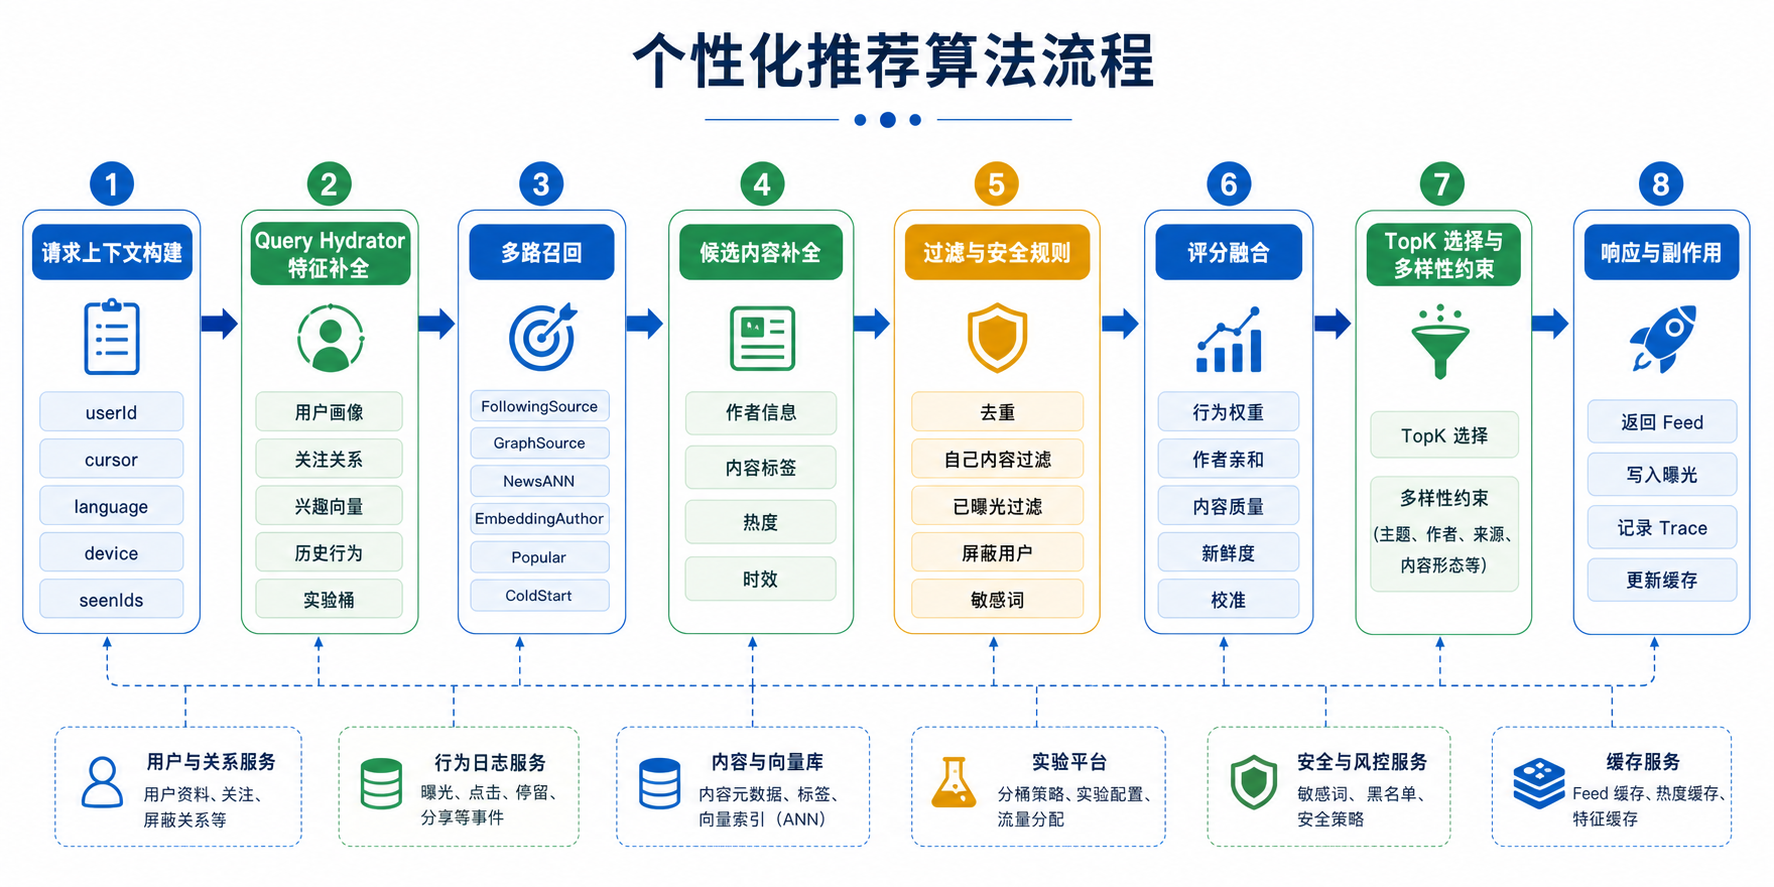
\includegraphics[width=0.98\textwidth]{recommendation-pipeline.png}
  \caption{个性化推荐算法流程图}
  \label{fig:recommendation_pipeline}
\end{figure}

\subsubsection{用户-内容交互建模}

推荐系统的本质是对用户$u \in \mathcal{U}$与内容$c \in \mathcal{C}$之间的潜在偏好进行估计。设用户在时刻$t$对内容$c$产生的行为为$y_{u,c,t}$，行为类型集合为

\[
\mathcal{A}=\{\text{impression}, \text{click}, \text{dwell}, \text{share}, \text{negative}\}
\]

其中曝光代表系统曾把内容展示给用户，点击、停留、分享属于正向反馈，不感兴趣、屏蔽、举报属于负向反馈。由于真实系统中绝大多数内容不会被用户显式评分，本项目采用隐式反馈建模思想，将行为强度映射为偏好置信度。对用户$u$和内容$c$，定义隐式偏好值：

\[
r_{u,c}=\sum_{a \in \mathcal{A}} \alpha_a \cdot n_{u,c}^{(a)}
\]

其中$n_{u,c}^{(a)}$表示行为$a$出现的次数，$\alpha_a$表示该行为的权重。点击权重较低，表示“有兴趣查看”；长停留、分享、回复权重较高，表示“深度兴趣”；负反馈权重为负，表示系统应该降低相似内容的排序。该思想与隐式反馈推荐和排序学习中的偏好强度建模一致\cite{hu2008collaborative,rendle2009bpr}。

为了同时表达用户的短期兴趣和长期兴趣，系统为每个用户维护两个向量：

\[
\mathbf{p}_u = \lambda \mathbf{p}_u^{short} + (1-\lambda)\mathbf{p}_u^{long}
\]

其中$\mathbf{p}_u^{short}$由最近点击、停留、分享的内容向量加权得到，更强调当前会话和近期兴趣；$\mathbf{p}_u^{long}$由较长时间窗口内的稳定行为得到，更强调长期偏好。$\lambda$是时间敏感系数，当用户近期行为密集时增大，当近期行为稀疏时减小。内容$c$的表示向量记为$\mathbf{q}_c$，可以由标题、摘要、关键词、分类和已有embedding字段综合得到。用户与内容的语义匹配分数定义为：

\[
s_{match}(u,c)=\cos(\mathbf{p}_u,\mathbf{q}_c)=
\frac{\mathbf{p}_u^\top \mathbf{q}_c}{\|\mathbf{p}_u\|_2\|\mathbf{q}_c\|_2}
\]

该得分用于向量召回和排序特征，能够弥补单纯社交关系召回无法发现新兴趣内容的问题。

\subsubsection{工程实现中的用户推荐特征清单}

为了便于复检，本项目将推荐算法使用的用户特征分为“持久化画像向量、实时行为信号、长期行为日志、社交图谱边、请求级上下文、候选评分特征”六类。前端只负责采集用户真实动作，后端再将动作转换为\texttt{user\_actions}、\texttt{user\_signals}、\texttt{real\_graph\_edges}和\texttt{user\_feature\_vectors}等推荐特征，不允许前端直接伪造兴趣向量或模型分数。

\begingroup
\hbadness=10000
\small
\begin{longtable}{L{0.17\textwidth}L{0.33\textwidth}L{0.39\textwidth}}
\toprule
特征层 & 主要字段 & 用途说明\\
\midrule
\endhead
持久化用户向量 & \texttt{interestedInClusters}、\texttt{knownForCluster}、\texttt{knownForScore}、\texttt{producerEmbedding} & 表示用户消费兴趣、生产者社区归属和作者侧稀疏向量，用于SimClusters式兴趣召回和作者匹配。\\
稠密Embedding & \texttt{twoTowerEmbedding}、\texttt{phoenixEmbedding}、\texttt{twhinEmbedding}、\texttt{embeddingDim} & 表示双塔、Phoenix和图嵌入空间中的用户向量，用于ANN召回、语义匹配和排序特征。\\
向量契约元数据 & \texttt{version}、\texttt{modelVersion}、\texttt{artifactVersion}、\texttt{modelProfile}、\texttt{embeddingContract}、\texttt{computedAt}、\texttt{expiresAt}、\texttt{qualityScore} & 记录向量由哪个模型和artifact生成、维度是否兼容、何时计算和是否过期，避免不同维度或不同版本向量混算。\\
实时用户信号 & \texttt{signalType}、\texttt{targetType}、\texttt{targetId}、\texttt{targetAuthorId}、\texttt{productSurface}、\texttt{metadata}、\texttt{timestamp}、\texttt{expiresAt} & 保存短期兴趣与负反馈，例如点击、停留、点赞、转发、引用、关注、不感兴趣、屏蔽、静音和举报，供实时特征聚合使用。\\
长期行为日志 & \texttt{action}、\texttt{targetPostId}、\texttt{targetAuthorId}、\texttt{requestId}、\texttt{rank}、\texttt{score}、\texttt{weightedScore}、\texttt{recallSource}、\texttt{selectionPool}、\texttt{targetKeywords}、\texttt{targetUrl} & 保存可回放、可审计的行为事实，用于训练样本、行为序列、推荐解释和线上问题追踪。\\
RealGraph社交边 & \texttt{followCount}、\texttt{likeCount}、\texttt{replyCount}、\texttt{retweetCount}、\texttt{quoteCount}、\texttt{tweetClickCount}、\texttt{dwellTimeMs}、\texttt{muteCount}、\texttt{blockCount}、\texttt{reportCount}、\texttt{decayedSum}、\texttt{interactionProbability} & 将用户与作者之间的互动累积为图边特征，正向互动增强作者亲和，静音、屏蔽、举报和取关降低或阻断关系分数。\\
请求级用户上下文 & \texttt{followedUserIds}、\texttt{blockedUserIds}、\texttt{mutedUserIds}、\texttt{mutedKeywords}、\texttt{seenPostIds}、\texttt{followerIds}、\texttt{userStateContext}、\texttt{userSignalFeatures}、\texttt{interestedTopics} & 在每次Feed请求开始时由Hydrator补齐，用于关注召回、屏蔽过滤、静音过滤、已看过滤、冷启动/稀疏/重度用户分层和兴趣话题匹配。\\
候选评分特征 & \texttt{likeScore}、\texttt{replyScore}、\texttt{repostScore}、\texttt{quoteScore}、\texttt{clickScore}、\texttt{profileClickScore}、\texttt{dwellScore}、\texttt{followAuthorScore}、\texttt{notInterestedScore}、\texttt{blockAuthorScore}、\texttt{muteAuthorScore}、\texttt{reportScore} & 对每条候选内容生成动作概率和负反馈概率。加权评分器对正向行为加分，对不感兴趣、屏蔽作者、静音作者和举报进行扣分。\\
\bottomrule
\end{longtable}
\endgroup

其中，\texttt{UserSignal}中的正权重信号包括点赞、转发、回复、引用、关注、分享、帖子点击、主页点击、外链点击、话题点击、搜索查询、曝光和停留；\texttt{QUOTE}按$+2.5$进入实时信号，并汇总为\texttt{UserSignalFeatures.quoteCount}和RealGraph的\texttt{quoteCount}。负权重信号包括取消点赞、取消转发、取消关注、屏蔽、静音、举报、取消书签和通知关闭，对应权重分别为$-0.5$、$-1.0$、$-3.0$、$-10.0$、$-5.0$、$-8.0$、$-0.5$和$-0.1$。\texttt{DISMISS\_POST}和\texttt{HIDE\_POST}虽然当前不在通用权重表中直接给出固定分值，但会写入\texttt{user\_actions}和\texttt{user\_signals}，并在候选负反馈特征、训练样本和Feed过滤/降权逻辑中使用。

\begingroup
\hbadness=10000
\scriptsize
\begin{longtable}{L{0.13\textwidth}L{0.20\textwidth}L{0.27\textwidth}L{0.26\textwidth}}
\toprule
正向/兴趣特征 & 前端入口 & 落库/接口 & 推荐侧影响\\
\midrule
\endhead
曝光与停留 & 帖子进入视口和可见停留计时 & \texttt{impression/dwell}埋点桥接到\path{user_actions}和\path{user_signals} & 形成served-history、行为序列和隐式兴趣强度。\\
帖子点击与主页点击 & 点击帖子卡片、头像或用户名 & \texttt{click/profile_click}埋点写入\texttt{ActionType.CLICK/PROFILE_CLICK}和对应\texttt{SignalType} & 增强内容兴趣和作者亲和，供Hydrator读取近期行为。\\
点赞、回复、转发 & 帖子操作栏按钮和评论抽屉 & \path{/like}、\path{/comments}、\path{/repost}写入推荐事件 & 增强显式兴趣、训练标签和RealGraph作者边。\\
引用动态 & 帖子更多菜单中的“引用动态”按钮，输入引用内容后发布 & \path{POST /api/space/posts}携带\texttt{quotePostId/quoteContent}，写入\texttt{ActionType.QUOTE}和\texttt{SignalType.QUOTE} & 进入\texttt{quoteCount}、\texttt{quoteScore}、Phoenix训练标签和RealGraph社交边。\\
分享与外链点击 & 分享按钮、Markdown外链 & 分享入口和\texttt{open_link}埋点写入\texttt{SignalType.SHARE/OPEN_LINK}，外链保留\texttt{targetUrl} & 作为轻量兴趣和内容传播信号。\\
搜索与话题点击 & 探索页搜索框、热门趋势和话题chip & \texttt{search_query/hashtag_click}桥接为\texttt{TargetType.SEARCH_QUERY/TOPIC} & 更新兴趣关键词和探索面意图。\\
关注 & 推荐关注卡片或个人主页关注按钮 & \path{POST /api/space/users/:id/follow}和analytics对账写入\texttt{SignalType.FOLLOW} & 进入关注召回、作者亲和和RealGraph。\\
\bottomrule
\end{longtable}
\endgroup

\begingroup
\hbadness=10000
\scriptsize
\begin{longtable}{L{0.13\textwidth}L{0.19\textwidth}L{0.25\textwidth}L{0.29\textwidth}}
\toprule
负向特征 & 前端入口 & 落库/接口 & 推荐侧影响\\
\midrule
\endhead
不感兴趣 & 帖子更多菜单中的“不感兴趣”按钮 & \path{/api/space/posts/:id/not-interested}，写入\path{ActionType.DISMISS}和\path{SignalType.DISMISS_POST} & 作为帖子级强负反馈，进入\path{notInterestedScore/dismissScore}和后续训练样本，降低相似内容排序。\\
隐藏帖子 & 帖子更多菜单中的“隐藏此帖”按钮 & \path{/api/space/posts/:id/hide}，写入\path{ActionType.HIDE}和\path{SignalType.HIDE_POST} & 当前请求中移除该帖子，并作为负反馈事实用于后续过滤、行为审计和训练。\\
举报 & 帖子更多菜单中的“举报”按钮，二级原因包含垃圾内容、骚扰、虚假信息、暴力仇恨和其他原因 & \path{/api/space/posts/:id/report}，写入\texttt{ActionType.REPORT}和\texttt{SignalType.REPORT} & 在\texttt{WeightedScorer}中按\texttt{REPORT\_WEIGHT=-8.0}扣分，同时进入RealGraph的\texttt{reportCount}。\\
屏蔽作者 & 帖子更多菜单中的“屏蔽 @作者”按钮 & \path{/api/space/users/:id/block}，写入联系人\texttt{blocked}状态和\texttt{SignalType.BLOCK} & 进入\texttt{blockedUserIds}硬过滤、\path{blockAuthorScore/blockScore}扣分和RealGraph的\texttt{blockCount}。\\
静音作者 & 帖子更多菜单中的“静音 @作者”按钮 & \path{/api/space/users/:id/mute}，写入用户设置和\texttt{SignalType.MUTE} & 进入\texttt{mutedUserIds}过滤、\texttt{muteAuthorScore}扣分和RealGraph的\texttt{muteCount}。\\
取消关注 & 推荐关注卡片或个人主页中的关注状态按钮，已关注时显示为“已关注”并可再次点击取消 & \texttt{DELETE} \path{/api/space/users/:id/follow}，写入\texttt{SignalType.UNFOLLOW} & 将作者关系从关注网络移除，并在RealGraph中减少\texttt{followCount}。\\
取消点赞 & 帖子点赞按钮的已点赞状态再次点击 & 前端埋点\texttt{unlike}映射到\path{SignalType.UNFAVORITE}，业务接口为\texttt{DELETE} \path{/api/space/posts/:id/like} & 作为轻度负向修正，降低用户对该内容/相似内容的偏好置信度。\\
取消转发 & 帖子转发按钮在已转发状态下显示为“取消转发”语义按钮 & \texttt{DELETE} \path{/api/space/posts/:id/repost}，写入\path{SignalType.UNRETWEET} & 与\texttt{UNRETWEET=-1.0}负权重对齐，作为撤销转发的轻度负反馈进入实时用户信号。\\
取消书签、通知关闭 & \texttt{UserSignal}权重表预留 & 当前Space Feed未提供书签和通知关闭入口 & 属于其他业务面或后续扩展字段，不应在Space演示中宣称已经由前端按钮采集。\\
\bottomrule
\end{longtable}
\endgroup

2026年6月11日通过Chrome DevTools MCP在生产前端\texttt{/space}页面进行只读复检：打开非本人作者\texttt{demo\_growth\_author\_06}的帖子更多菜单后，页面DOM中实际存在“不感兴趣”“隐藏此帖”“举报”“屏蔽 @demo\_growth\_author\_06”“静音 @demo\_growth\_author\_06”五个按钮；进入举报二级菜单后，实际存在“垃圾内容/广告”“骚扰/霸凌”“虚假信息”“暴力/仇恨”“其他原因”五个原因按钮。本次复检没有点击最终提交类按钮，网络请求中未出现\texttt{/not-interested}、\texttt{/hide}、\texttt{/report}、\texttt{/block}或\texttt{/mute}写接口，因此不会污染线上用户特征。取消转发闭环在代码和组件测试中补齐：当帖子处于已转发状态时，同一转发按钮的语义变为“取消转发”，并调用\texttt{DELETE /api/space/posts/:id/repost}写入\texttt{UNRETWEET}。引用闭环在本轮补齐：更多菜单新增“引用动态”入口，前端提交引用文本后调用\texttt{POST /api/space/posts}并携带\texttt{quotePostId}，后端写入\texttt{QUOTE}推荐事件。当前前端没有“拉踩”或\texttt{downvote/dislike}按钮，对应算法也未定义独立拉踩特征；演示时应将“不感兴趣、隐藏、举报、屏蔽、静音、取消转发、取消点赞、取消关注”作为负向减分入口。

\subsubsection{多路召回模型}

多路召回阶段的目标是在可控延迟内从海量内容集合$\mathcal{C}$中构造较小候选集$\mathcal{R}_u$。如果直接对所有内容排序，时间复杂度为$O(|\mathcal{C}|)$，在实际Feed场景中不可接受。因此系统将召回看作多个弱检索器的并集：

\[
\mathcal{R}_u = \bigcup_{m=1}^{M} \mathcal{R}_u^{(m)}
\]

其中$m$表示召回通道，$\mathcal{R}_u^{(m)}$表示第$m$路召回结果。每一路召回承担不同的信息增益：

\begin{enumerate}
  \item \textbf{关注召回}：从用户关注对象的时间线中读取近期内容，适合关注关系稳定的用户。
  \item \textbf{社交图谱召回}：根据共同联系人、共同群组和互动关系扩展候选作者。
  \item \textbf{新闻向量召回}：利用内容关键词和向量特征查找相似新闻。
  \item \textbf{作者兴趣召回}：根据用户长期兴趣向量匹配更可能感兴趣的作者。
  \item \textbf{热门召回}：选取近期点击、分享、停留表现较好的内容。
  \item \textbf{冷启动召回}：当用户行为较少时，使用地区、语言和全局热度生成候选。
\end{enumerate}

从概率角度看，每一路召回都近似估计一个条件概率$P(c|u,m)$。关注召回强调$P(c|follow(u))$，社交图谱召回强调$P(c|G_u)$，向量召回强调$P(c|\mathbf{p}_u)$，热门召回强调$P(c|global)$。最终候选集并不是简单平均，而是根据用户状态动态调整各路配额。设用户状态为$z_u \in \{\text{cold},\text{sparse},\text{warm},\text{heavy}\}$，第$m$路召回配额为：

\[
K_m(u)=K \cdot \frac{\pi_m(z_u)\cdot h_m}{\sum_{j=1}^{M}\pi_j(z_u)\cdot h_j}
\]

其中$K$表示总候选规模，$\pi_m(z_u)$表示不同用户状态下的召回偏好，$h_m$表示召回源健康度。对于冷启动用户，热门召回和地区语言召回权重更高；对于重度用户，关注召回、向量召回和作者亲和召回权重更高。该设计可以避免“新用户无结果”和“老用户结果过于热门化”两个常见问题。

\subsubsection{规则过滤与约束建模}

召回阶段追求覆盖率，过滤阶段追求安全性和有效性。设召回候选为$\mathcal{R}_u$，过滤后候选为$\mathcal{F}_u$，则：

\[
\mathcal{F}_u=\{c \in \mathcal{R}_u \mid g_k(u,c)=1,\; k=1,2,\dots,L\}
\]

其中$g_k$是第$k$个硬约束函数。系统中主要约束包括：去重约束、已曝光过滤、自身内容过滤、屏蔽用户过滤、敏感词过滤、内容时效过滤和重复转发过滤。硬约束的优先级高于模型得分，因为违反这些规则会直接损害用户体验或平台安全。

对已曝光内容，系统维护集合$\mathcal{E}_u$，如果$c \in \mathcal{E}_u$，则过滤该内容或显著降低得分。该机制解决推荐系统中的重复曝光问题。对负反馈内容，系统不仅过滤具体内容，还会将负反馈传播到相似作者、相似主题和相似关键词：

\[
penalty(u,c)=\beta_1 I(author(c)\in B_u)+\beta_2 sim(topic(c),T_u^{-})+\beta_3 sim(keyword(c),K_u^{-})
\]

其中$B_u$表示用户屏蔽作者集合，$T_u^{-}$表示负反馈主题集合，$K_u^{-}$表示负反馈关键词集合。该惩罚项进入排序阶段，避免系统反复推荐用户明确拒绝的内容。

\subsubsection{排序评分函数}

评分阶段采用可解释的多目标融合模型。设候选内容$c$对用户$u$的最终得分为$S(u,c)$，可表示为：

\[
S(u,c)=w_1E(u,c)+w_2A(u,c)+w_3Q(c)+w_4R(c)+w_5M(u,c)-w_6N(u,c)
\]

其中，$E(u,c)$表示用户行为兴趣得分，$A(u,c)$表示作者亲和度，$Q(c)$表示内容质量，$R(c)$表示新鲜度，$M(u,c)$表示语义匹配得分，$N(u,c)$表示负反馈惩罚项。权重$w_i$可以由实验配置控制，也可以在后续通过学习排序模型自动学习。

各部分含义如下：

\begin{enumerate}
  \item \textbf{行为兴趣得分}：由点击、停留、分享、回复等行为加权得到，表达用户对相似内容的历史偏好。
  \item \textbf{作者亲和度}：由关注关系、共同群组、历史互动、作者内容点击率等特征构成，衡量用户与作者之间的社交距离。
  \item \textbf{内容质量}：由内容完整度、来源可信度、历史互动率和负反馈率构成，避免低质量内容因短期热度被过度放大。
  \item \textbf{新鲜度}：使用时间衰减函数计算，保证Feed具备实时性。
  \item \textbf{语义匹配}：使用用户兴趣向量与内容向量余弦相似度计算，表达主题层面的匹配程度。
  \item \textbf{负反馈惩罚}：由屏蔽、不感兴趣、举报、关键词厌恶等信号组成，用于降低不符合用户偏好的内容。
\end{enumerate}

新鲜度采用指数衰减模型：

\[
R(c)=\exp\left(-\frac{t_{now}-t_c}{\tau}\right)
\]

其中$t_c$为内容发布时间，$\tau$为时间半衰参数。新闻类内容对新鲜度敏感，$\tau$应较小；知识类或长期有效内容对新鲜度不敏感，$\tau$可以增大。该函数可以避免旧内容长期占据高位，同时不会让刚发布但质量很低的内容无条件排在前面。

行为兴趣得分采用归一化加权形式：

\[
E(u,c)=\sigma\left(\sum_{a \in \mathcal{A}^{+}}\alpha_a f_a(u,c)-\sum_{b \in \mathcal{A}^{-}}\gamma_b f_b(u,c)\right)
\]

其中$\sigma(x)=1/(1+e^{-x})$为Sigmoid函数，$\mathcal{A}^{+}$为正向行为集合，$\mathcal{A}^{-}$为负向行为集合。使用Sigmoid的原因是将原始行为强度压缩到$[0,1]$区间，避免某个高频行为单独支配排序。

\subsubsection{排序校准与多样性重排}

如果直接按照$S(u,c)$取TopK，系统容易出现“信息茧房”和“作者集中”问题。为此，最终选择阶段采用带多样性约束的贪心重排。设已选择集合为$\mathcal{S}$，下一条内容$c^\ast$满足：

\[
c^\ast=\arg\max_{c \in \mathcal{F}_u \setminus \mathcal{S}}
\left[S(u,c)-\eta \max_{c' \in \mathcal{S}} sim(c,c')\right]
\]

其中$sim(c,c')$表示两个内容在作者、主题、来源或向量空间中的相似度，$\eta$为多样性惩罚系数。该公式与最大边际相关性（MMR）思想一致\cite{carbonell1998mmr}。当已选择列表中存在同主题内容时，相似候选会被惩罚，从而提升推荐列表的信息覆盖面。

同时，系统对不同召回来源进行校准。由于热门召回天然具有较高互动数，向量召回天然更贴近兴趣但可能互动较少，若不校准会导致某一路召回长期占优。系统引入来源校准项：

\[
S'(u,c)=S(u,c)+\delta_{source(c)}+\delta_{bucket(u)}
\]

其中$\delta_{source(c)}$用于修正不同召回源的系统性偏差，$\delta_{bucket(u)}$用于支持实验分桶。这样既可以做工程上的灰度实验，也可以在报告层面体现推荐算法的可观测和可调优能力。

\subsubsection{目标函数与评价指标}

从优化目标看，推荐系统不是单纯最大化点击率，而是多目标优化问题。系统希望同时提升点击、停留、分享和满意度，并降低负反馈。因此可定义总体效用函数：

\[
J=\mathbb{E}_{(u,c)\sim \mathcal{D}}
\left[\theta_1 click+\theta_2 dwell+\theta_3 share-\theta_4 negative-\theta_5 latency\right]
\]

其中$\mathcal{D}$为线上请求分布，$latency$表示推荐接口延迟。该目标函数体现了课程项目中的工程权衡：推荐结果要相关，但接口也要稳定、快速、可解释。离线评估可以使用Precision@K、Recall@K、NDCG@K和覆盖率；在线评估可以使用CTR、平均停留时长、分享率、负反馈率和P95延迟。实验表中的\texttt{experiments}表正是为后续A/B测试准备的。

综合来看，本项目推荐算法并非只按热度排序，而是形成了“特征建模--多路召回--规则过滤--多目标排序--多样性重排--实验评估”的完整闭环。该闭环与工业推荐系统和经典深度推荐模型的设计思想一致\cite{covington,cheng,he2017ncf}，同时保留了课程项目需要的可解释性与工程可实现性。

\subsection{数据库设计}

通过Supabase MCP读取可知，本项目云端数据库项目为\texttt{telegram}，核心表结构如图\ref{fig:supabase_er_diagram}所示。数据库主要分为基础社交模块、推荐内容模块和实验平台模块。

\begin{figure}[htbp]
  \centering
  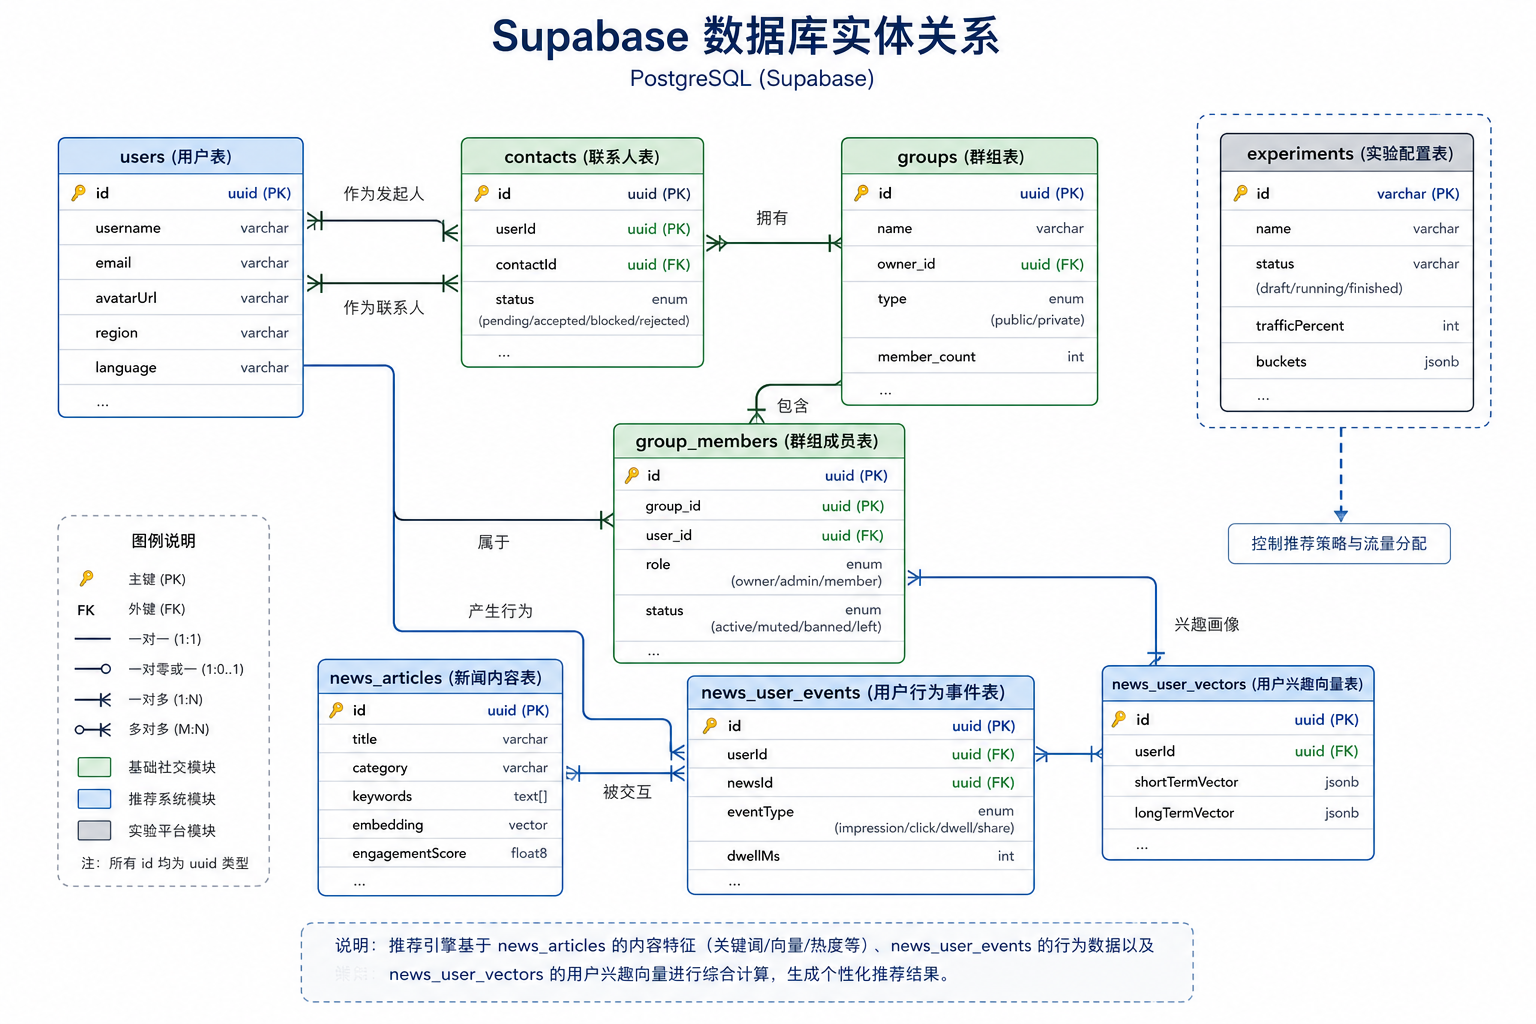
\includegraphics[width=0.95\textwidth]{supabase-er-diagram.png}
  \caption{Supabase数据库实体关系图}
  \label{fig:supabase_er_diagram}
\end{figure}

\begin{longtable}{L{0.25\textwidth}L{0.18\textwidth}L{0.48\textwidth}}
\caption{核心数据表说明}\\
\toprule
表名 & 当前记录数 & 用途说明 \\
\midrule
\endfirsthead
\toprule
表名 & 当前记录数 & 用途说明 \\
\midrule
\endhead
\texttt{users} & 642 & 保存用户编号、用户名、邮箱、头像、地区、语言和在线状态。\\
\texttt{groups} & 6 & 保存群组名称、描述、群主、类型、成员数量和最大成员数。\\
\texttt{group\_members} & 764 & 保存用户与群组的成员关系、角色、状态和加入时间。\\
\texttt{contacts} & 195 & 保存联系人关系、联系人状态和备注名。\\
\texttt{news\_articles} & 838 & 保存新闻标题、摘要、来源、分类、关键词、向量、互动计数和有效状态。\\
\texttt{news\_user\_events} & 2386 & 保存曝光、点击、停留、分享等用户行为事件。\\
\texttt{news\_user\_vectors} & 6 & 保存用户短期兴趣向量和长期兴趣向量。\\
\texttt{experiments} & 2 & 保存推荐实验名称、状态、流量比例、分桶方式和评价指标。\\
\bottomrule
\end{longtable}

\subsection{接口设计}

系统核心接口设计如下：

\begin{longtable}{L{0.13\textwidth}L{0.34\textwidth}L{0.41\textwidth}}
\caption{核心接口设计}\\
\toprule
方法 & 路径 & 说明 \\
\midrule
\endfirsthead
\toprule
方法 & 路径 & 说明 \\
\midrule
\endhead
GET & \path{/api/space/feed} & 获取个性化推荐Feed，支持分页、数量限制和是否只看关注内容。\\
POST & \path{/api/space/feed} & 携带已曝光内容、请求编号和客户端上下文获取Feed。\\
GET & \path{/api/space/trends} & 获取趋势主题和热门内容。\\
GET & \path{/api/space/recommend/users} & 推荐可能感兴趣的用户或作者。\\
POST & \path{/api/events/news} & 上报曝光、点击、停留、分享等行为事件。\\
\bottomrule
\end{longtable}

\subsection{安全设计}

安全设计主要包括接口鉴权、参数校验、数据库访问控制和敏感字段保护。Spring Boot后端使用JWT识别当前用户，推荐接口只允许登录用户访问。请求参数如\texttt{limit}需要设置上限，避免一次请求拉取过多候选内容。涉及密码、用户行为和兴趣向量的数据不应直接暴露给前端。

需要特别说明的是，Supabase安全检查发现当前公开模式下多张表尚未启用RLS，包括\texttt{users}、\texttt{groups}、\texttt{contacts}、\texttt{news\_articles}、\texttt{news\_user\_events}等。课程报告中将其作为部署安全风险记录，实际上线前应启用RLS并补充按用户、角色和服务端密钥区分的访问策略。

\section{本章小结}

本章完成了项目的需求分析、可行性分析、架构设计、模块设计、推荐算法流程设计、数据库设计和接口设计。系统以Spring Boot作为后端核心，以Supabase PostgreSQL作为云端数据库，以Redis提升缓存性能，以Apifox支撑接口联调。推荐算法采用多路召回、规则过滤、加权评分和TopK选择的分层流程，能够满足课程大作业对分布式架构和推荐系统思想的要求。

% !TeX root = ../thuthesis-example.tex

\chapter{项目测试}

\section{测试环境}

本项目测试围绕接口联调、数据库结构检查和推荐算法流程检查展开。测试环境如下：

\begin{longtable}{p{0.28\textwidth}p{0.62\textwidth}}
\caption{测试环境说明}\\
\toprule
项目 & 说明 \\
\midrule
\endfirsthead
\toprule
项目 & 说明 \\
\midrule
\endhead
后端框架 & Spring Boot后端设计，接口按RESTful风格组织。\\
接口工具 & Apifox桌面端，用于构造请求、解析参数和保存联调截图。\\
数据库 & Supabase PostgreSQL，项目名\texttt{telegram}，区域\texttt{us-west-2}。\\
缓存设计 & Redis，用于时间线缓存、热点Feed缓存和临时特征缓存。\\
测试接口 & 推荐Feed接口、趋势接口、用户推荐接口、行为事件接口。\\
\bottomrule
\end{longtable}

\section{Apifox接口联调}

在Apifox中创建快捷请求，分别对推荐Feed、趋势内容、用户推荐和主题内容接口进行参数联调。推荐Feed接口测试地址设计为：

\begin{center}
\texttt{http://localhost:8080/api/space/feed?limit=10\&in\_network\_only=false}
\end{center}

Apifox会自动将URL中的查询参数解析到Params区域，其中\texttt{limit=10}表示本次请求最多返回10条推荐内容，\texttt{in\_network\_only=false}表示允许系统从关注关系以外的召回源获取内容。联调界面如图\ref{fig:apifox_feed_request}所示。

\begin{figure}[htbp]
  \centering
  \begin{minipage}{0.48\textwidth}
    \centering
    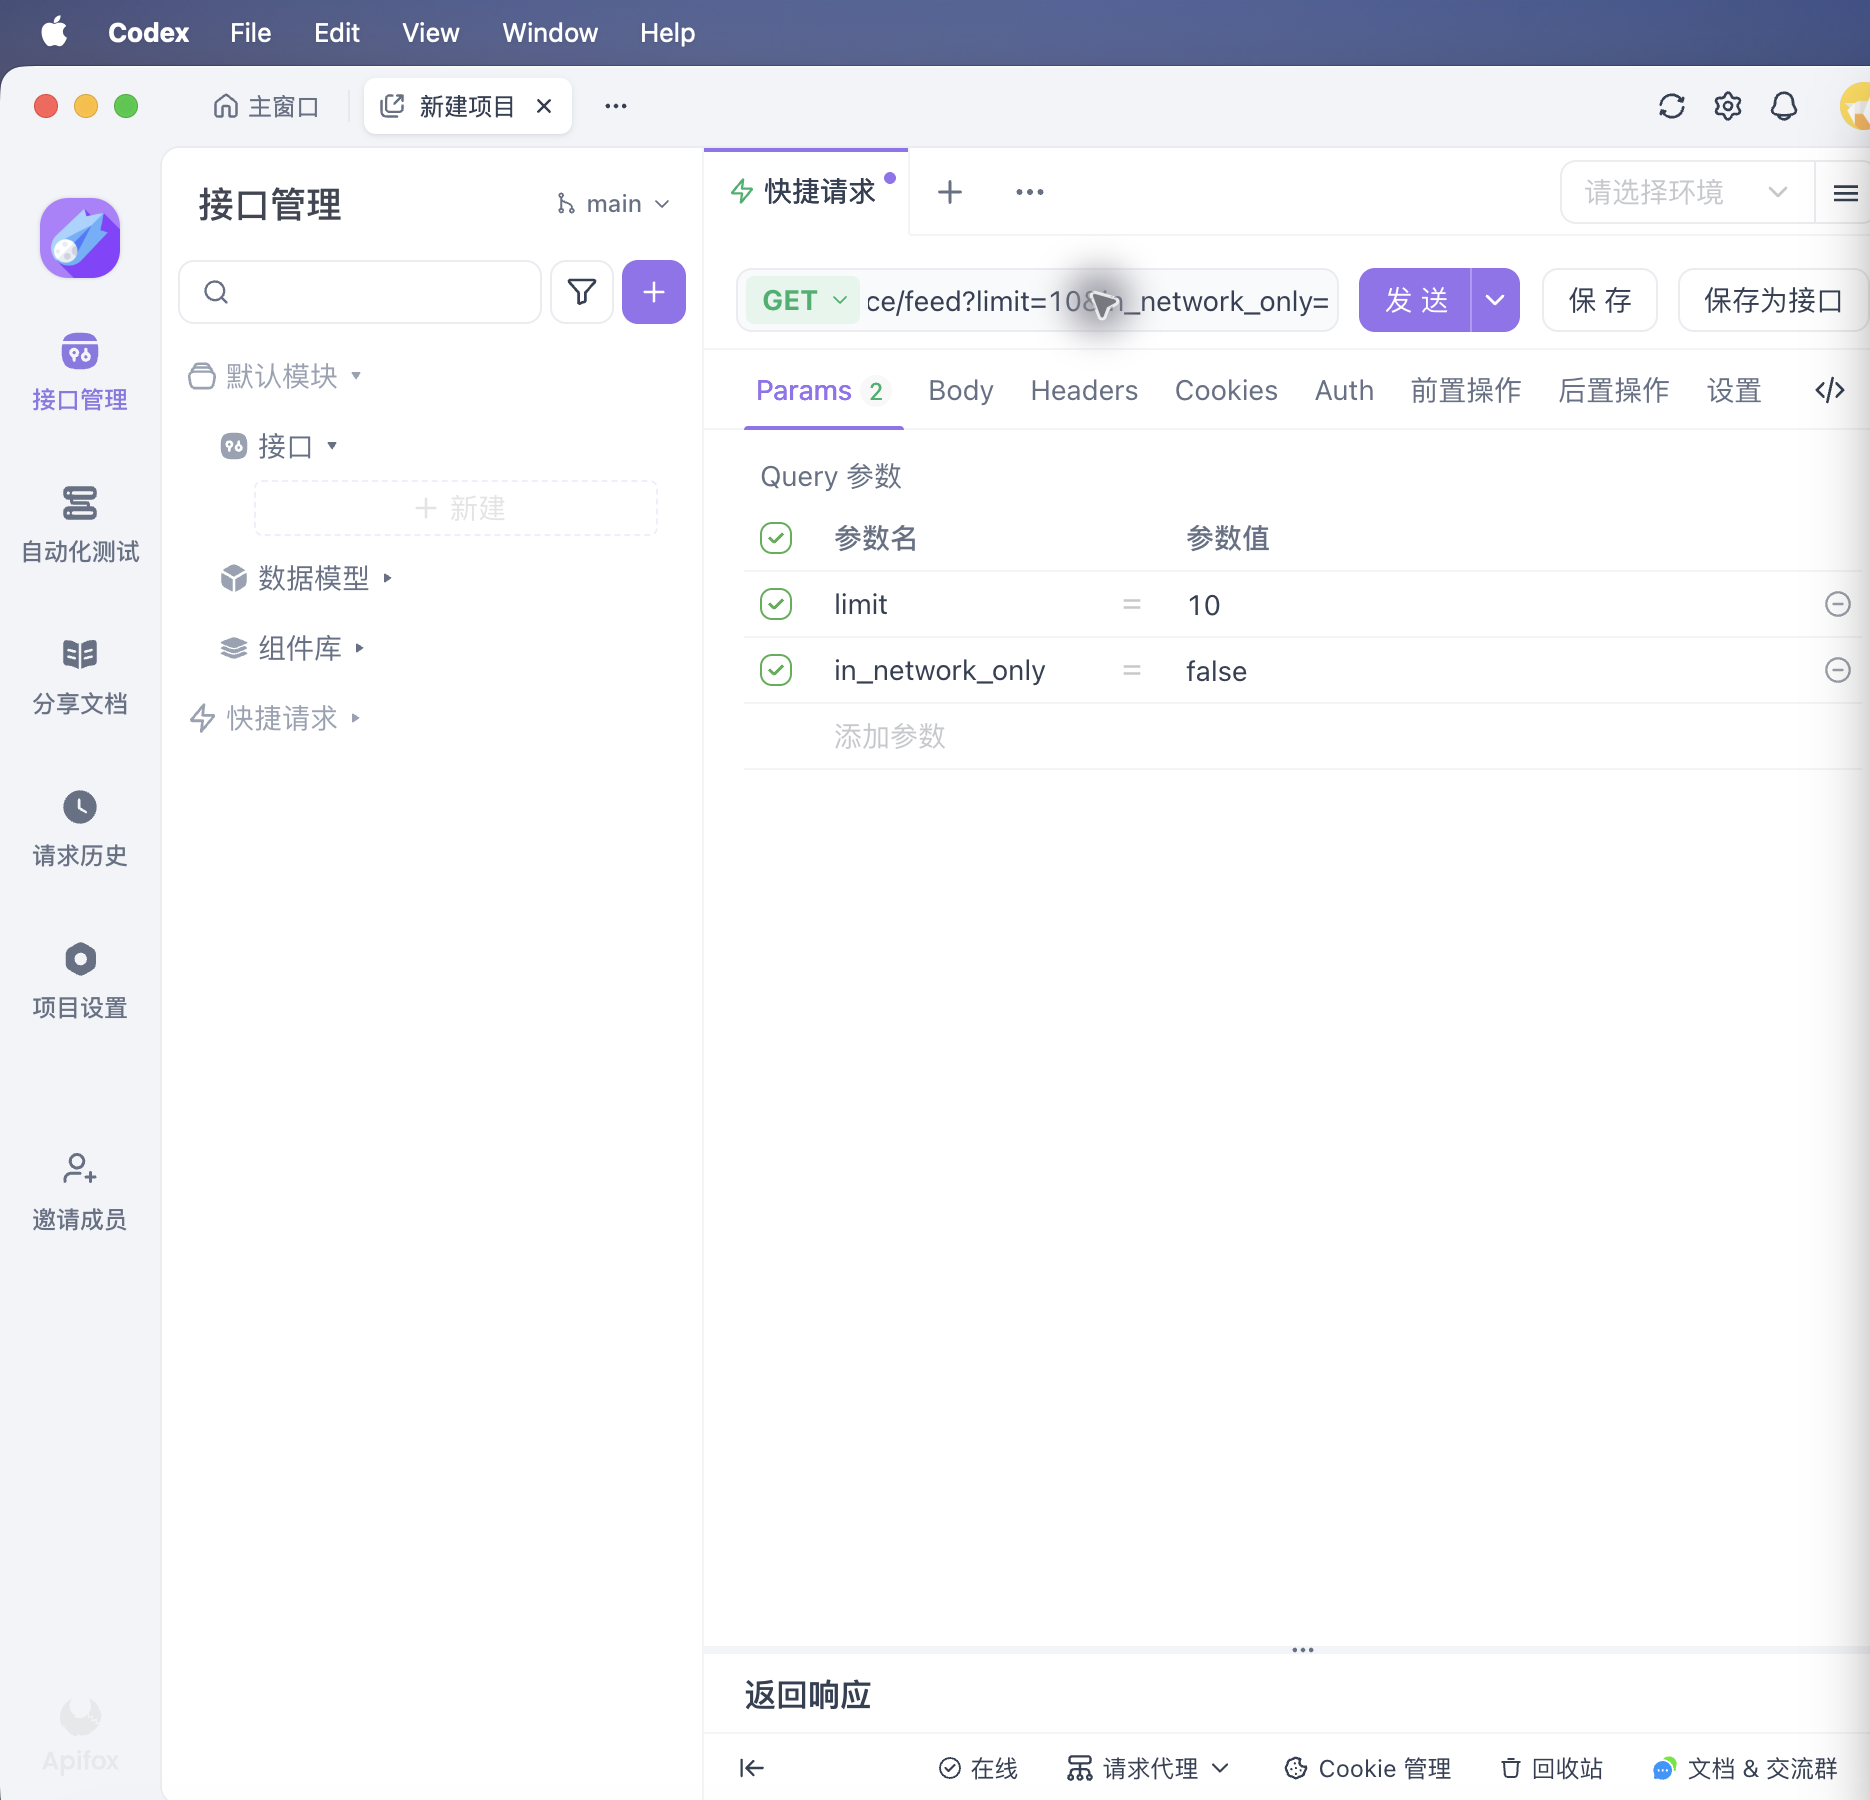
\includegraphics[width=\linewidth]{apifox-feed-request-cropped.png}\\
    {\small （a）推荐Feed接口参数联调}
  \end{minipage}
  \hfill
  \begin{minipage}{0.48\textwidth}
    \centering
    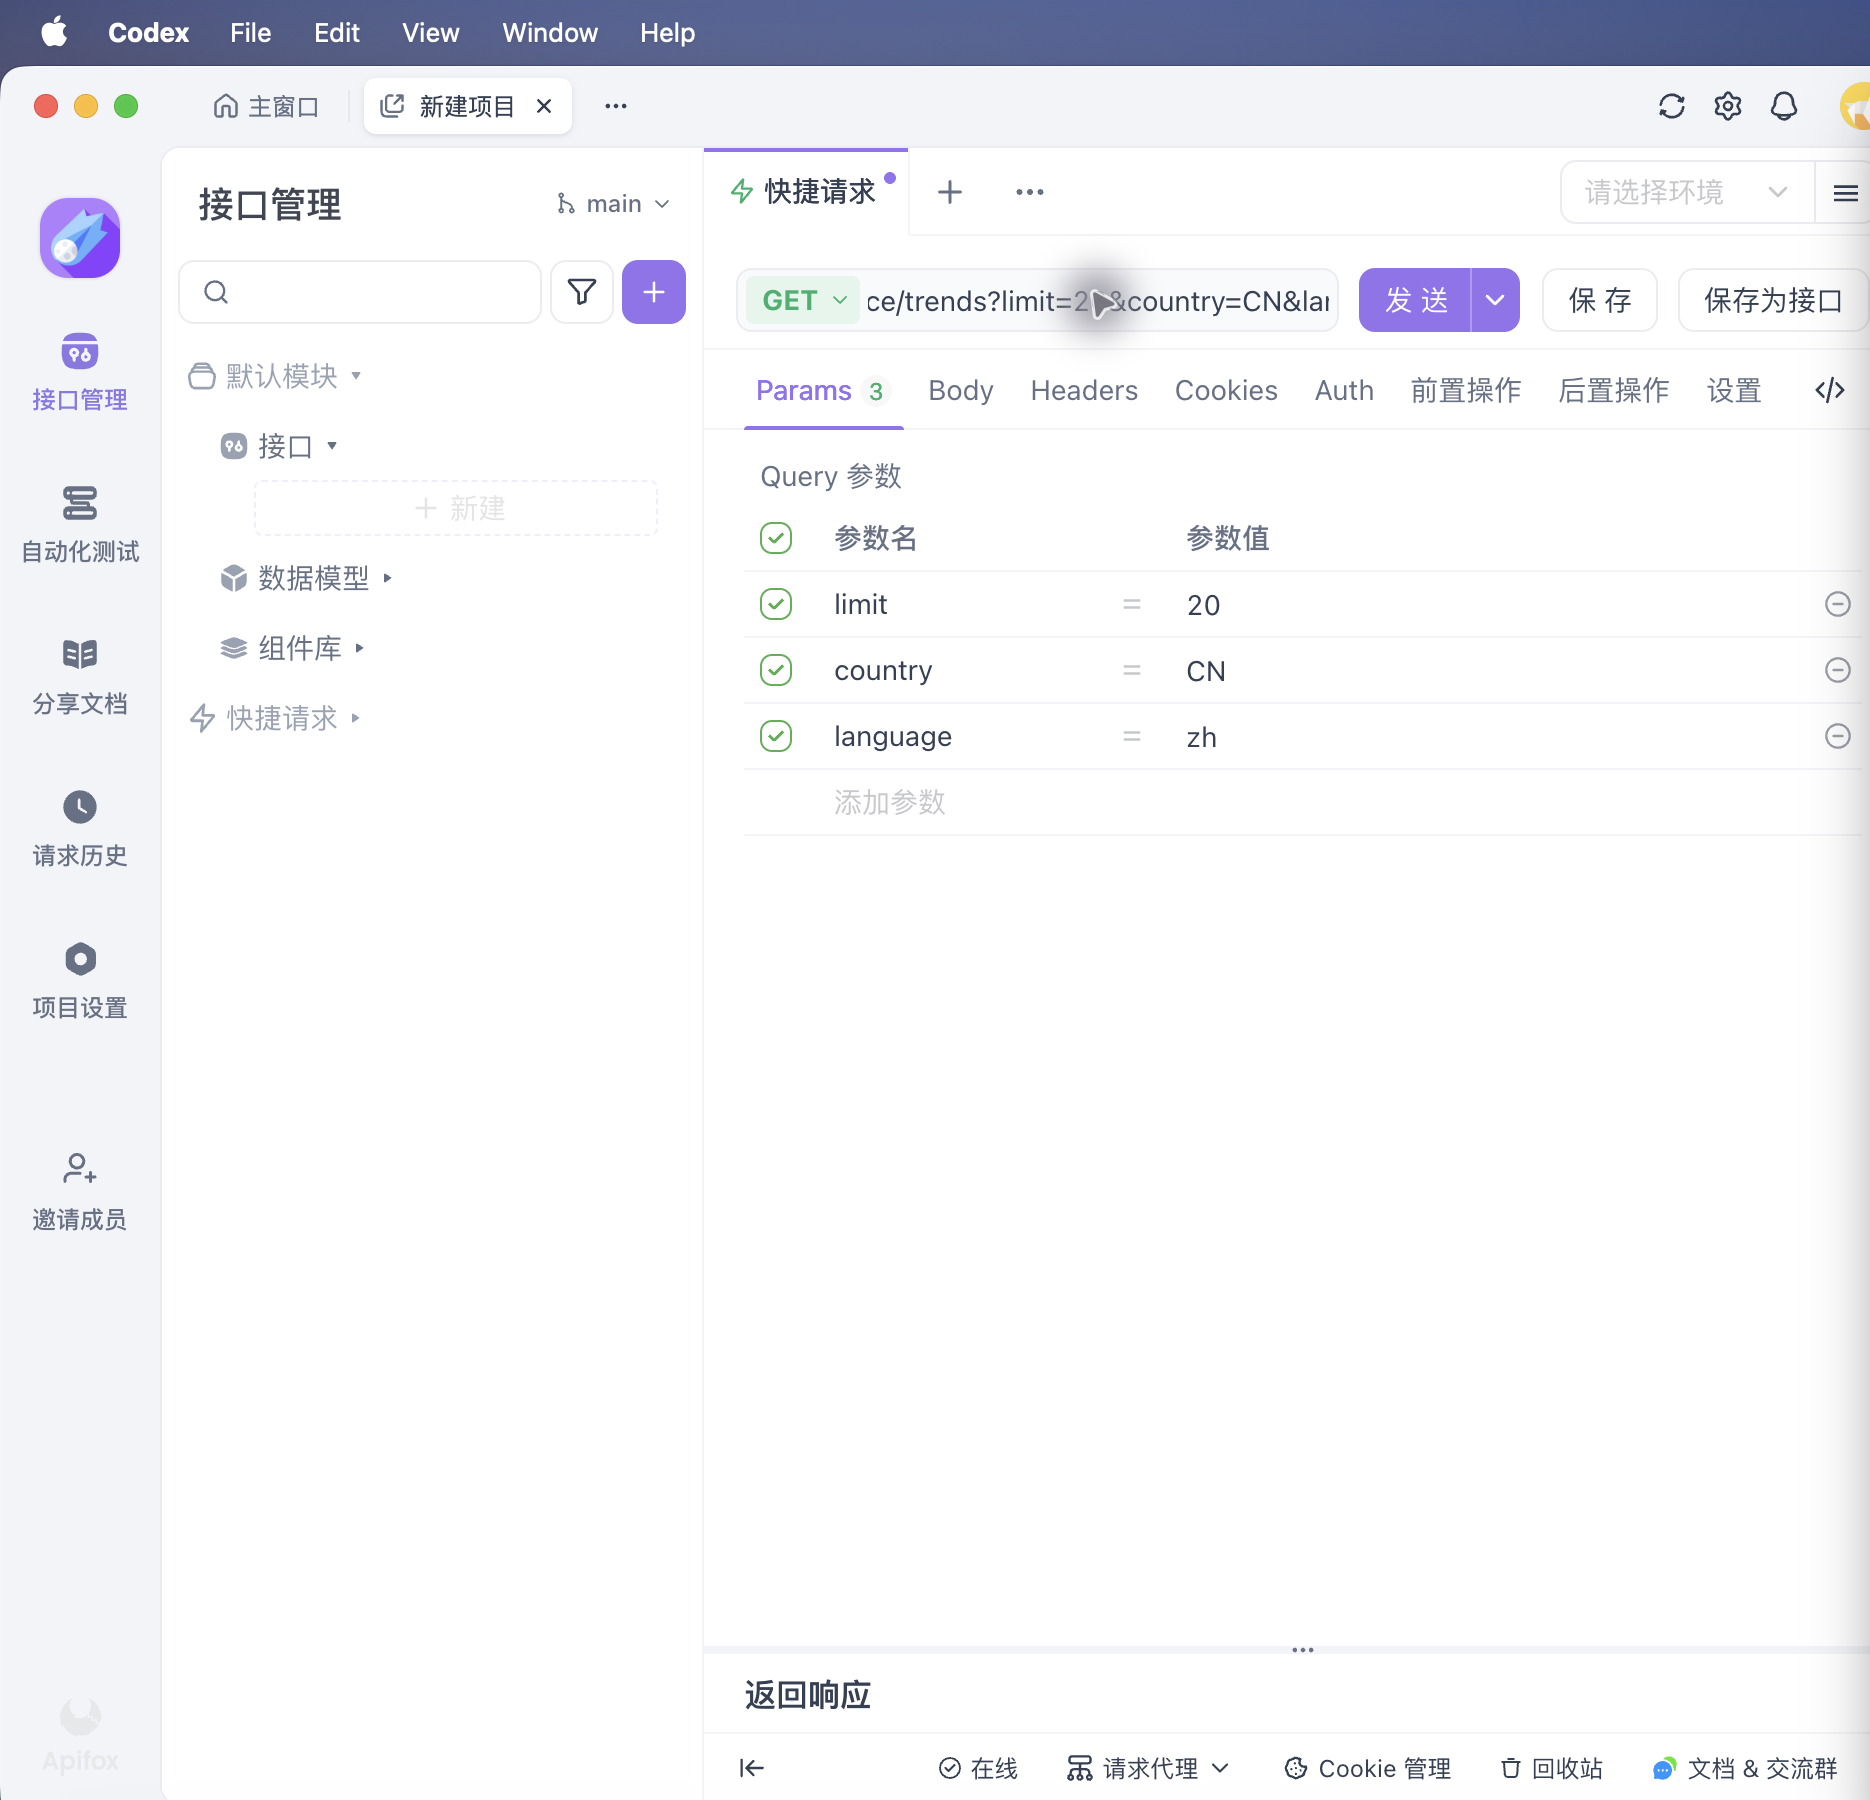
\includegraphics[width=\linewidth]{apifox-trends-request-cropped.png}\\
    {\small （b）趋势内容接口参数联调}
  \end{minipage}

  \vspace{0.35cm}

  \begin{minipage}{0.48\textwidth}
    \centering
    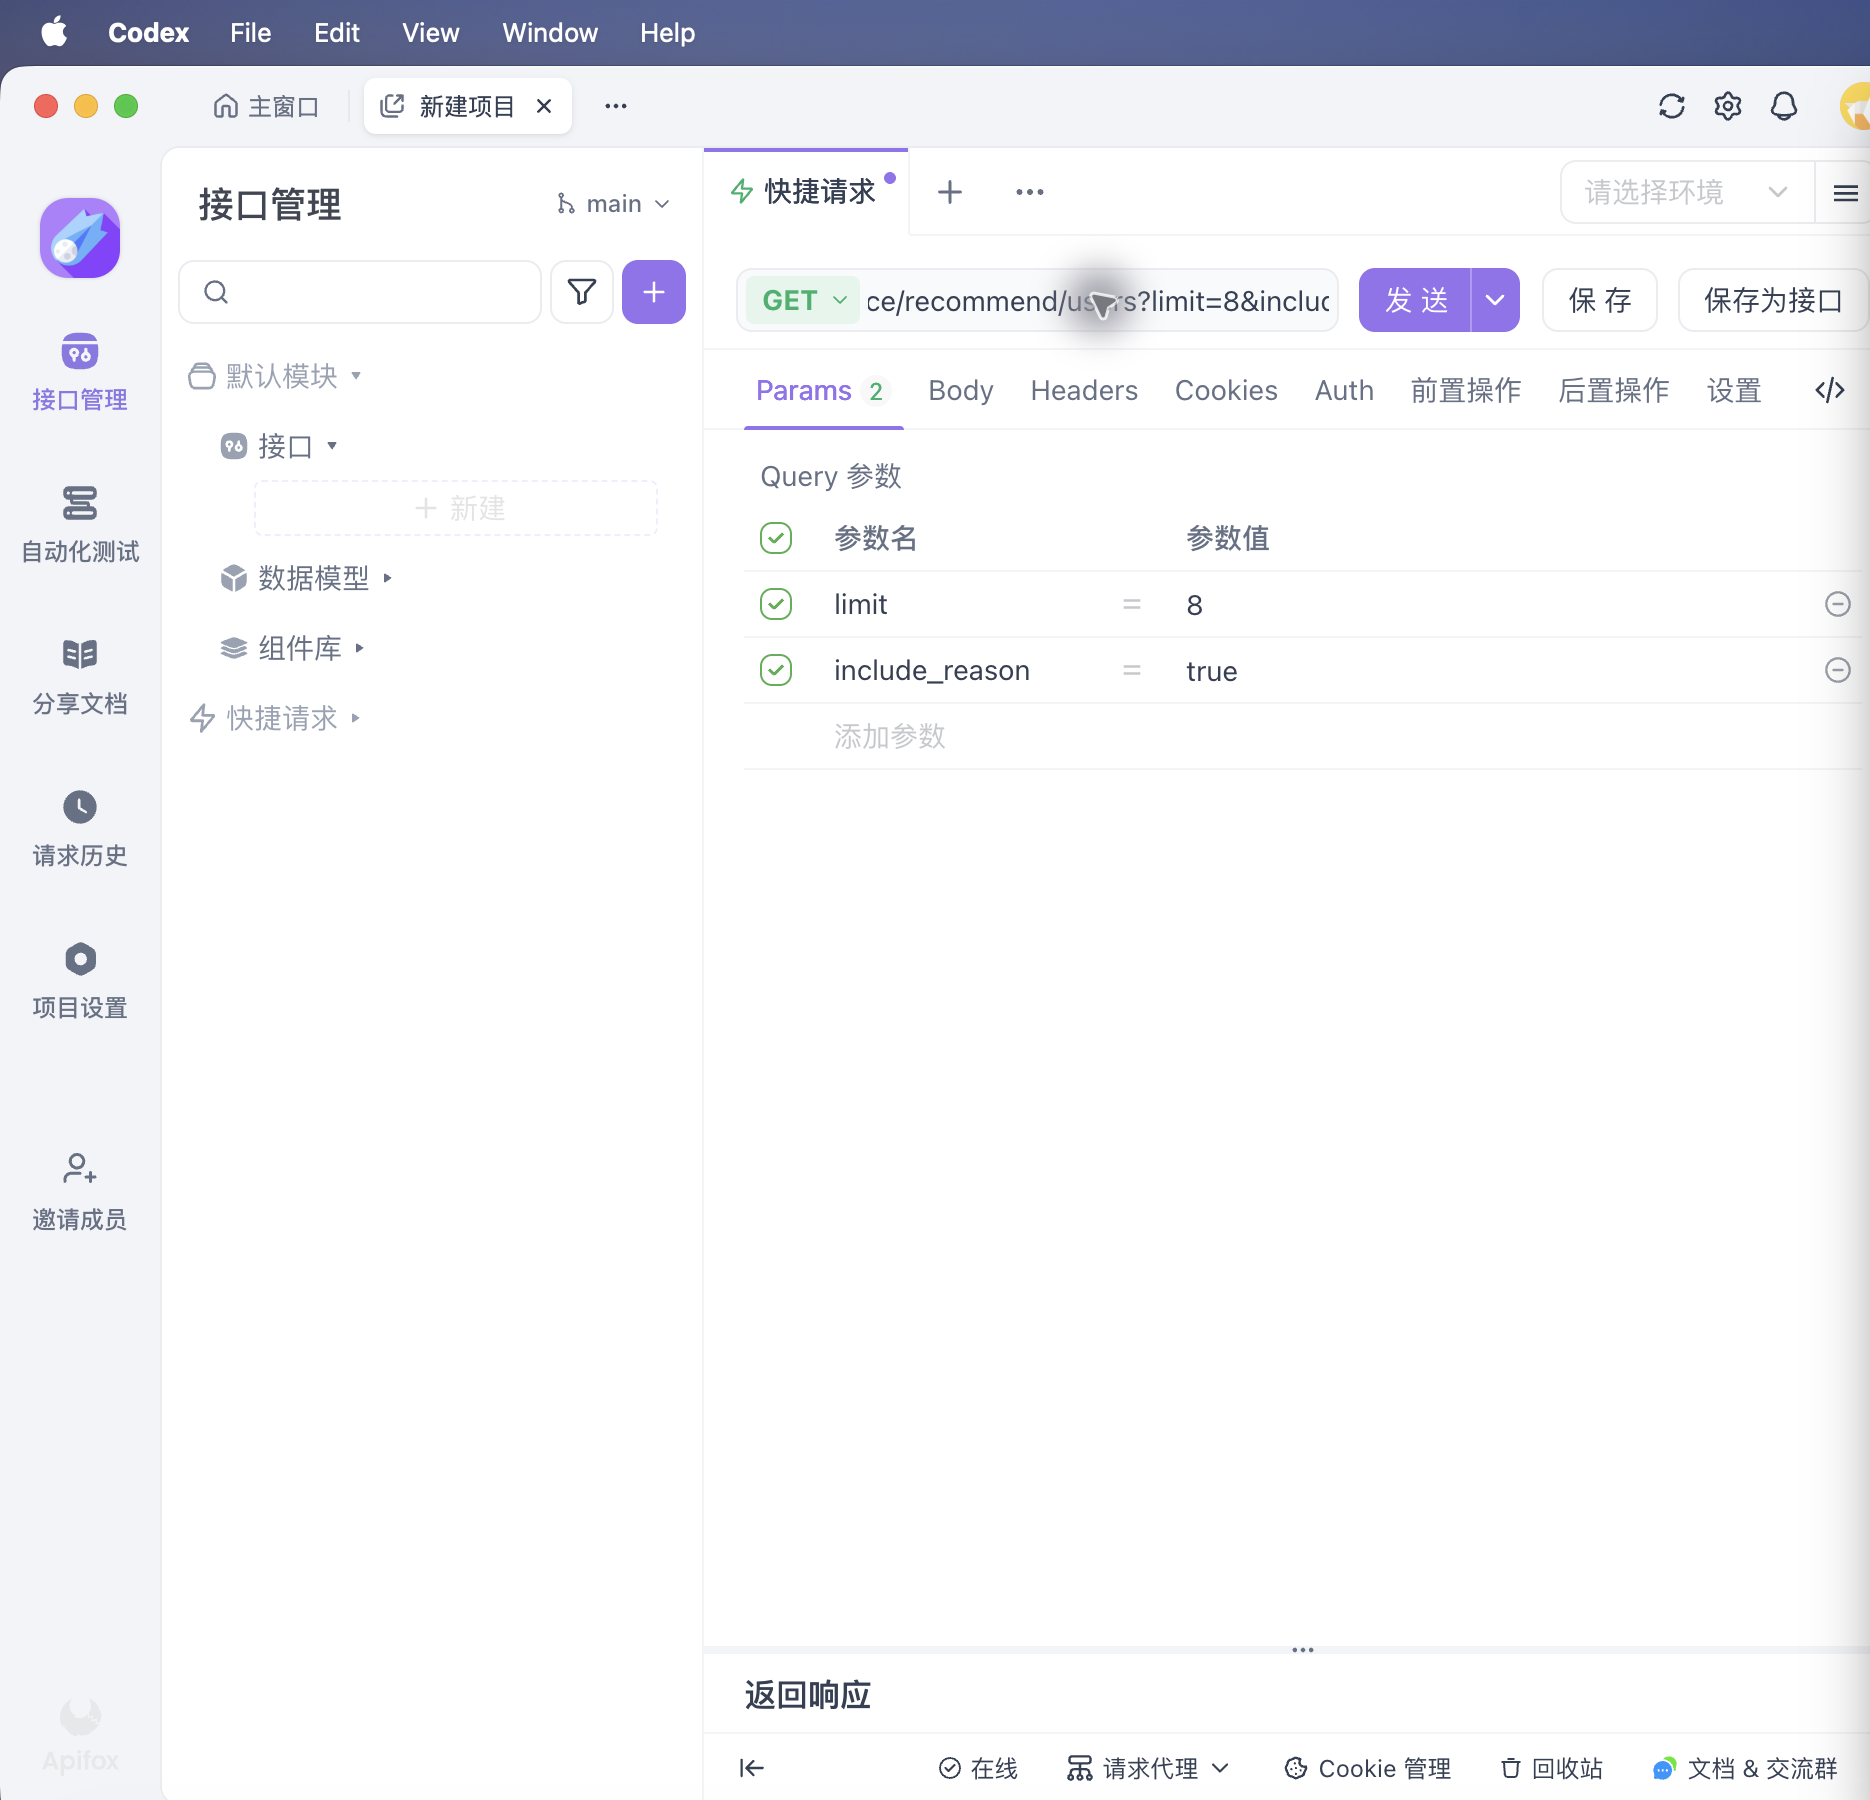
\includegraphics[width=\linewidth]{apifox-users-request-cropped.png}\\
    {\small （c）用户推荐接口参数联调}
  \end{minipage}
  \hfill
  \begin{minipage}{0.48\textwidth}
    \centering
    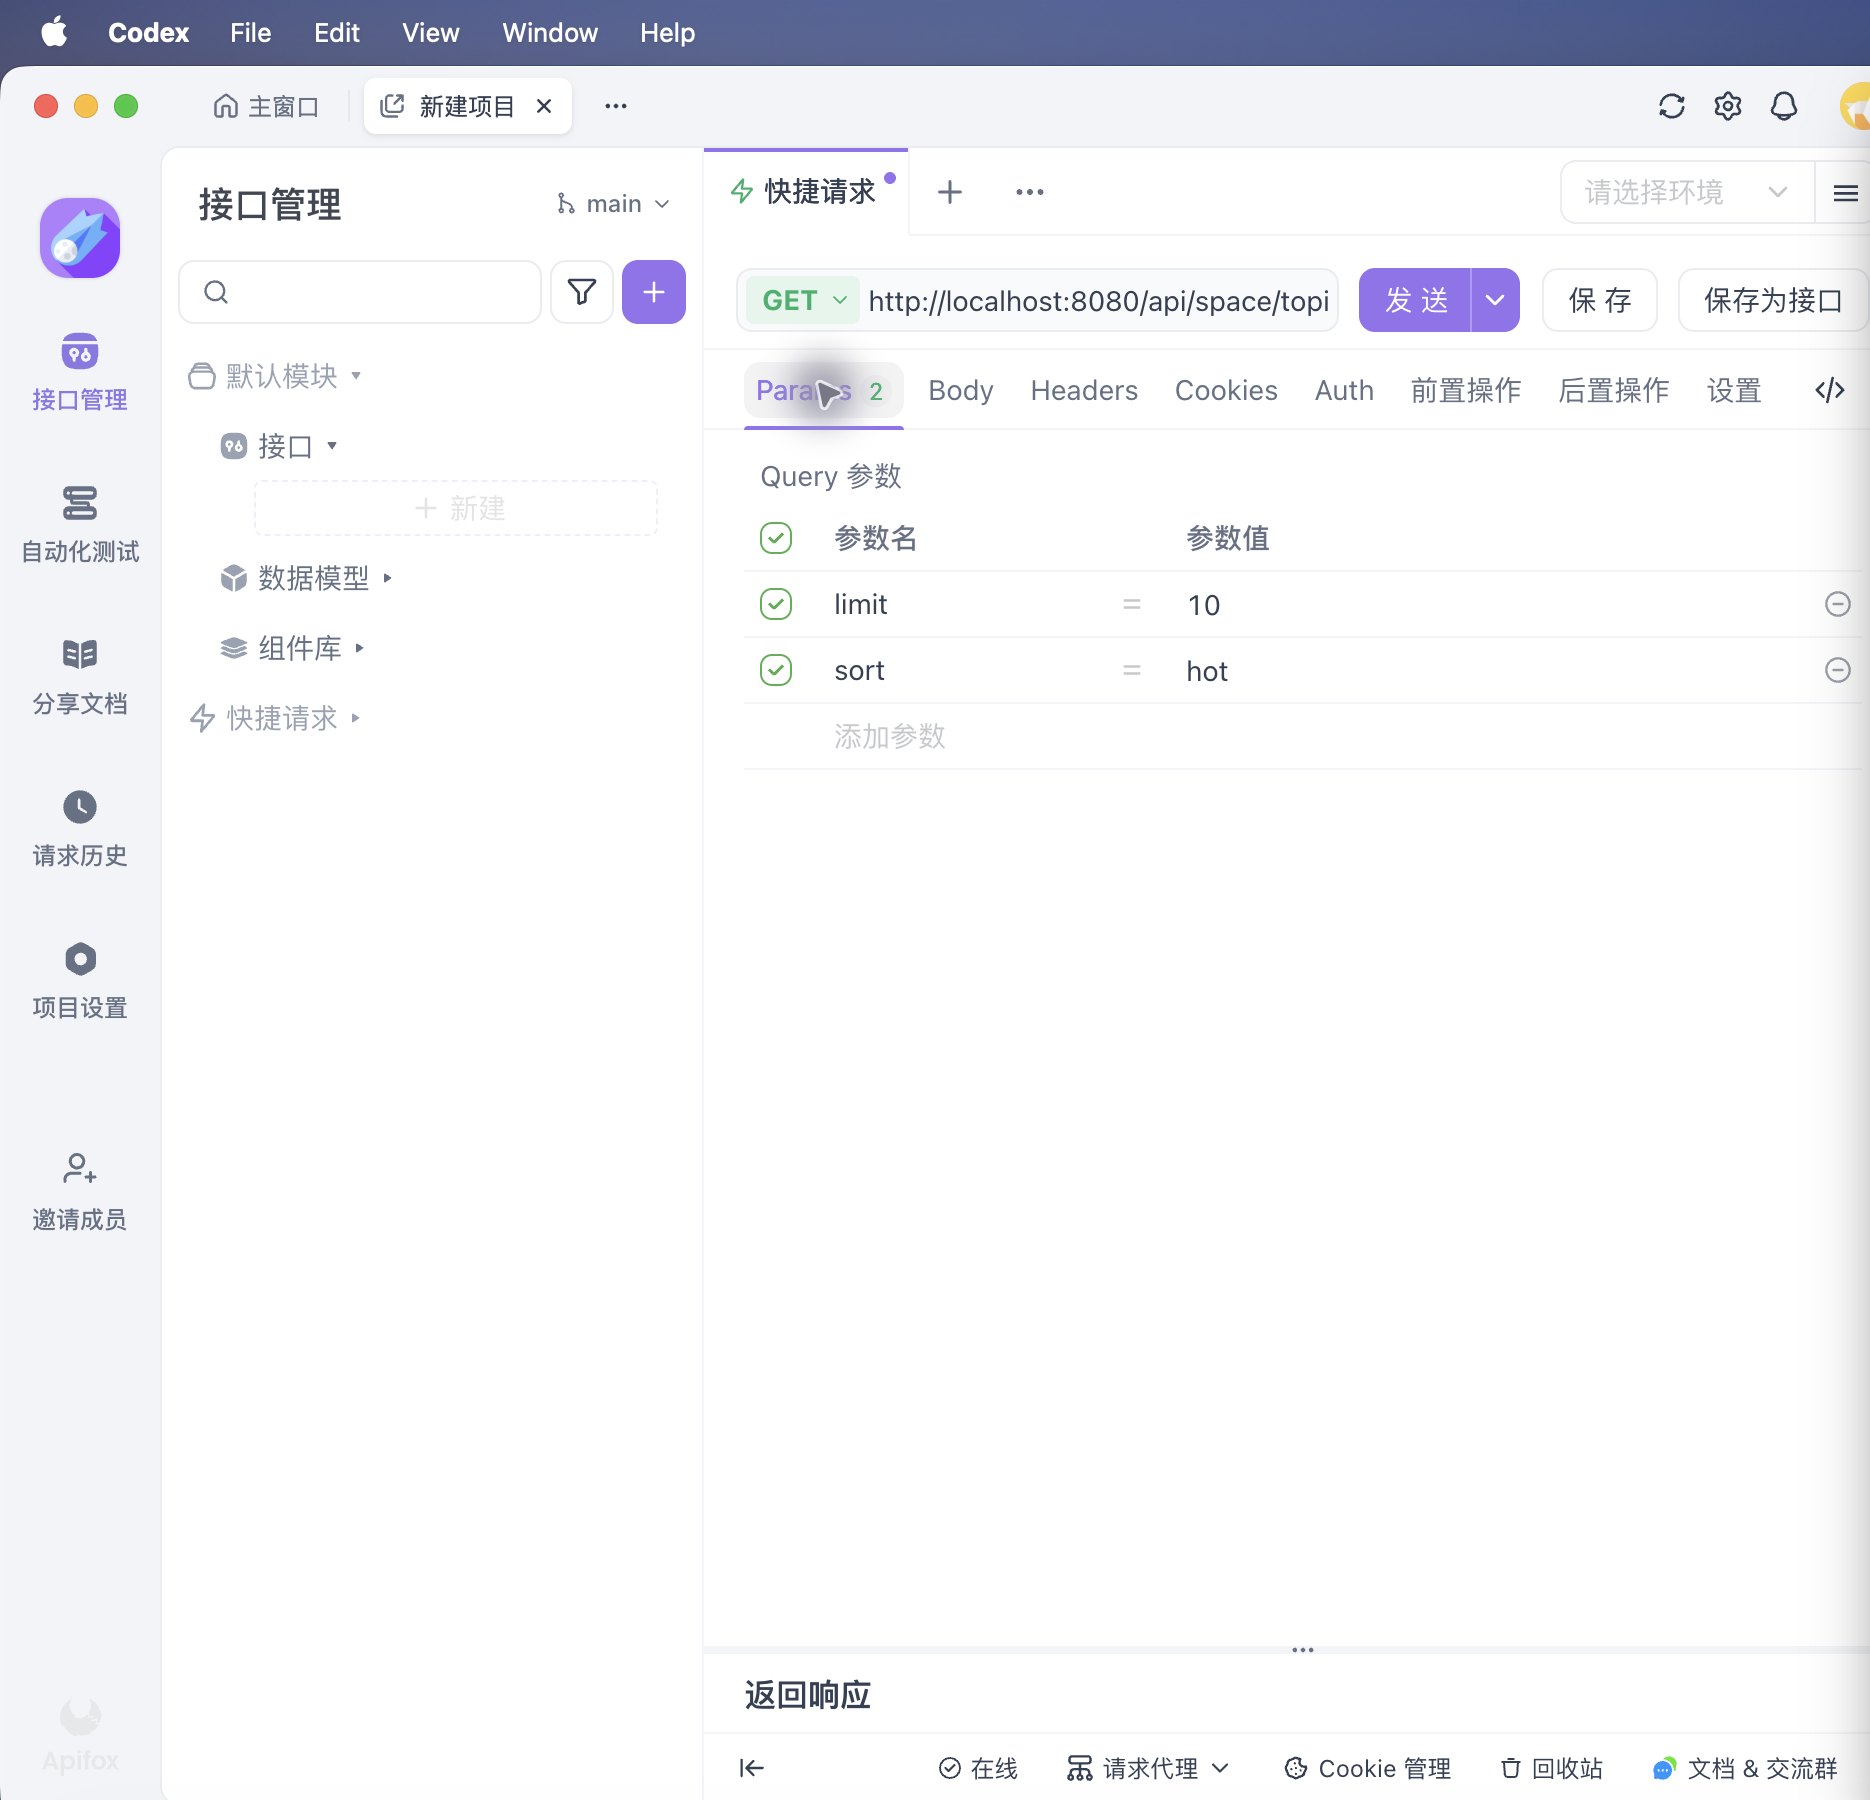
\includegraphics[width=\linewidth]{apifox-topic-request-cropped.png}\\
    {\small （d）主题内容接口参数联调}
  \end{minipage}
  \caption{Apifox多接口联调截图}
  \label{fig:apifox_feed_request}
\end{figure}

图\ref{fig:apifox_feed_request}展示了四类接口的联调准备。推荐Feed接口用于验证个性化内容流，趋势内容接口用于验证按国家和语言过滤的热点内容，用户推荐接口用于验证用户关系扩展能力，主题内容接口用于验证按话题聚合内容。四张截图均显示Apifox已经将URL中的查询参数解析为表格，便于逐项检查参数名、参数值和接口路径。后续接入真实运行的Spring Boot服务后，可以继续补充Authorization请求头、JSON响应断言和自动化测试集合。

\section{核心接口测试用例}

\begin{longtable}{p{0.2\textwidth}p{0.3\textwidth}p{0.36\textwidth}}
\caption{核心接口测试用例}\\
\toprule
测试项 & 输入 & 预期结果 \\
\midrule
\endfirsthead
\toprule
测试项 & 输入 & 预期结果 \\
\midrule
\endhead
推荐Feed接口 & \texttt{limit=10}，允许站外召回 & 返回不超过10条内容，包含内容编号、标题、作者、来源和分页游标。\\
关注内Feed & \texttt{in\_network\_only=true} & 候选内容优先来自关注作者或直接社交关系。\\
冷启动Feed & 新用户或行为较少用户 & 返回热门内容、地区语言匹配内容和冷启动内容。\\
趋势接口 & 无特殊参数 & 返回近期互动较高的话题、新闻或作者。\\
用户推荐接口 & 当前登录用户编号 & 返回可能感兴趣的用户，避免推荐自己和已屏蔽用户。\\
行为事件接口 & 点击、停留、分享事件 & 事件写入\texttt{news\_user\_events}，可用于兴趣向量更新。\\
\bottomrule
\end{longtable}

\section{数据库检查}

通过Supabase MCP读取数据库结构，确认项目\texttt{telegram}处于\texttt{ACTIVE\_HEALTHY}状态，数据库主机为Supabase托管PostgreSQL。核心业务表均已存在，且具备推荐系统所需数据基础。

数据库检查结果如下：

\begin{enumerate}
  \item 用户与社交关系数据充足。\texttt{users}表有642条记录，\texttt{group\_members}表有764条记录，\texttt{contacts}表有195条记录，可支撑社交召回。
  \item 内容数据具备推荐基础。\texttt{news\_articles}表有838条记录，包含标题、摘要、分类、关键词、向量和互动计数等字段。
  \item 行为数据可用于排序。\texttt{news\_user\_events}表有2386条记录，事件类型包括曝光、点击、停留和分享。
  \item 用户兴趣向量表已存在。\texttt{news\_user\_vectors}表保存短期向量和长期向量，可用于个性化匹配。
  \item 实验配置表已存在。\texttt{experiments}表有2条记录，可用于A/B测试和推荐策略灰度。
\end{enumerate}

\section{推荐算法测试}

推荐算法测试重点不是单个函数是否返回固定值，而是检查推荐流水线是否能覆盖不同用户状态。测试设计如下：

\begin{enumerate}
  \item 冷启动用户测试：当用户没有足够行为时，系统应减少兴趣向量依赖，优先使用热门内容、语言地区匹配和冷启动召回。
  \item 稀疏行为用户测试：当用户有少量关注和点击记录时，系统应同时使用社交图谱召回和热门召回，避免结果过窄。
  \item 活跃用户测试：当用户有较多行为事件和兴趣向量时，系统应提高向量召回、作者亲和和内容质量得分的影响。
  \item 负反馈测试：当用户屏蔽作者、标记不感兴趣或已曝光某内容时，过滤阶段应将其剔除或显著降权。
  \item 多样性测试：当多个候选来自同一作者或同一主题时，TopK选择阶段应控制重复度。
\end{enumerate}

\section{测试结论}

根据Apifox联调界面、Supabase数据库结构和推荐算法流程检查，可以认为本项目具备课程设计要求的主要测试证据：接口路径明确、请求参数可解析、云端数据库真实存在、推荐算法流程完整、核心数据表能够支撑用户关系和内容行为分析。

同时，测试中发现Supabase公开模式下多张表尚未启用RLS，其中\texttt{users}表还包含\texttt{password}字段。该问题不影响课程报告的结构撰写，但属于真实上线前必须处理的安全风险。建议在正式部署前启用RLS，并将密码字段改为不可逆哈希存储，禁止前端直接访问敏感表。

% !TeX root = ../thuthesis-example.tex

\chapter{总结与展望}

\section{总结}

本文完成了“基于Spring Boot的分布式推荐系统”的课程大作业报告撰写。系统以类Telegram社交应用为业务背景，将后端设计为Spring Boot分层架构，前端负责页面展示和行为采集，Supabase PostgreSQL负责云端数据持久化，Redis负责缓存与时间线加速，Apifox负责接口联调。

在系统设计方面，本文按照课程模板完成了需求分析、可行性分析、系统架构设计、模块设计、数据库设计和接口设计。系统整体分为客户端层、后端服务层、数据与缓存层和推荐算法层。后端模块包括认证与权限、用户与群组、新闻内容、推荐Feed、行为埋点和实验配置。该设计避免了将所有逻辑堆叠在单一接口中，体现了分布式应用的模块边界意识。

在推荐算法方面，本文重点描述了多阶段推荐流水线。系统先构建请求上下文，再补全用户画像和实验信息，随后通过关注关系、社交图谱、新闻向量、作者兴趣、热门内容和冷启动内容进行多路召回。候选内容进入过滤阶段后，会去除重复、自身内容、已曝光内容、屏蔽用户和敏感词。评分阶段综合行为权重、作者亲和度、内容质量、新鲜度和负反馈惩罚，最终通过TopK选择生成个性化Feed。

在测试方面，本文使用Apifox完成推荐Feed接口的请求配置截图，并通过Supabase MCP读取真实云端数据库结构。数据库中已存在用户、群组、联系人、新闻内容、用户行为、用户兴趣向量和实验配置等表，能够支撑推荐系统的基本数据需求。

\section{展望}

虽然本项目已经形成完整的课程报告和系统设计，但距离真实生产级推荐系统仍有改进空间。

首先，后端可以从单体Spring Boot多模块架构逐步演进为微服务架构。推荐服务、用户服务、内容服务、实验服务和日志服务可以独立部署，通过服务注册、网关和熔断机制提高系统可维护性。

其次，推荐算法可以从规则加权模型升级为可训练模型。当前设计重点强调可解释性和工程可落地性，后续可以引入双塔模型、矩阵分解、图神经网络或Learning to Rank模型，根据真实行为数据自动学习权重。

第三，行为数据闭环仍需加强。后续可以建立离线特征计算任务，定期根据点击、停留、分享和负反馈更新用户兴趣向量，并将模型指标接入实验平台。

第四，安全策略需要完善。Supabase当前存在公开表未启用RLS的问题，真实上线前应启用行级安全策略，补充按用户身份、管理员角色和服务端密钥区分的访问规则，同时对密码字段进行哈希存储和脱敏处理。

最后，测试体系可以进一步自动化。Apifox当前主要用于手动联调和截图记录，后续可增加响应断言、环境变量、前置脚本和自动化测试集合，使接口测试能够随着后端迭代持续执行。

% !TeX root = ../thuthesis-example.tex

\chapter*{致谢}
\addcontentsline{toc}{chapter}{致谢}

在本次分布式应用技术课程大作业完成过程中，感谢指导教师江亮老师在课程要求、技术方向和项目规范方面给予的指导。通过本次项目，我们进一步理解了Spring Boot后端开发、云端数据库、接口联调、前后端分离和推荐系统设计之间的关系。

同时，感谢小组成员在资料整理、数据库检查、接口测试、算法设计和报告撰写中的协作。本项目从封面格式、章节结构到系统架构图、推荐流程图和数据库说明均按照课程模板进行整理，使最终报告能够较完整地呈现项目设计过程。

最后，感谢开源社区提供的Spring Boot、React、PostgreSQL、Redis、Supabase和Apifox等工具与技术资料。这些工具降低了分布式应用原型设计和课程展示的实现成本，也为后续继续完善项目提供了基础。

% 参考文献
\nocite{*}
\bibliography{ref/refs}  % 参考文献使用 BibTeX 编译
% \printbibliography       % 参考文献使用 BibLaTeX 编译

% 附录
%\appendix
%% !TeX root = ./thuthesis-example.tex

\chapter{源代码}
\begin{cpp}
	#include "mbed.h"

// ==========================================
// 1. 硬件引脚定义
// ==========================================

// --- 数码管 ---
DigitalOut segA(p13); DigitalOut segB(p14); DigitalOut segC(p15);
DigitalOut segD(p16); DigitalOut segE(p17); DigitalOut segF(p18);
DigitalOut segG(p19); DigitalOut segDP(p20);
DigitalOut digitLeft(p23); DigitalOut digitMid(p22); DigitalOut digitRight(p21);

// --- 交通灯定义 (外部引脚) ---
// 东西向
DigitalOut ew_red(p25);
DigitalOut ew_yellow(p26);
DigitalOut ew_green(p27);

// 南北向
DigitalOut ns_red(p28);
DigitalOut ns_yellow(p29);
DigitalOut ns_green(p30);

// --- 行人灯 ---
DigitalOut ped_blue(p24);  // 蓝灯: 通行
DigitalOut ped_white(p12); // 白灯: 禁行

// --- 按键扫描 (S1) ---
DigitalIn row1(p5, PullUp); 
DigitalOut col1(p9); 

// ==========================================
// 2. 全局变量 & 状态定义
// ==========================================

enum TrafficState {
    ST_EW_GO,    // 东西绿
    ST_EW_WARN,  // 东西黄
    ST_NS_GO,    // 南北绿
    ST_NS_WARN,  // 南北黄
    ST_PED_WALK  // 行人通行
};

TrafficState current_state = ST_EW_GO;
int countdown = 0;        
bool ped_request = false; 

// 自定义时长 (秒)
#define TIME_EW_GO    15 
#define TIME_EW_WARN  3   
#define TIME_NS_GO    10 
#define TIME_NS_WARN  3   
#define TIME_PED_WALK 10  

Timer sys_timer;
float last_tick = 0;

// 数码管段码
const int digitPatterns[10][7] = {
    {1,1,1,1,1,1,0}, {0,1,1,0,0,0,0}, {1,1,0,1,1,0,1}, {1,1,1,1,0,0,1},
    {0,1,1,0,0,1,1}, {1,0,1,1,0,1,1}, {1,0,1,1,1,1,1}, {1,1,1,0,0,0,0},
    {1,1,1,1,1,1,1}, {1,1,1,1,0,1,1}
};

// ==========================================
// 3. 驱动函数
// ==========================================

void setSegments(int idx) {
    if (idx < 0 || idx > 9) { 
        segA=0; segB=0; segC=0; segD=0; segE=0; segF=0; segG=0; segDP=0; return;
    }
    segA=digitPatterns[idx][0]; segB=digitPatterns[idx][1]; segC=digitPatterns[idx][2];
    segD=digitPatterns[idx][3]; segE=digitPatterns[idx][4]; segF=digitPatterns[idx][5];
    segG=digitPatterns[idx][6]; segDP=0;
}

void clearDisplay() {
    digitLeft=1; digitMid=1; digitRight=1;
    segA=0; segB=0; segC=0; segD=0; segE=0; segF=0; segG=0; segDP=0;
}

void refresh_display() {
    int num = countdown;
    if (num < 0) num = 0;
    
    if (num >= 10) {
        setSegments(num / 10); digitLeft = 0; wait_us(2000); clearDisplay();
    }
    setSegments(num % 10); digitMid = 0; wait_us(2000); clearDisplay();
}

bool is_button_pressed() {
    col1 = 0; 
    wait_us(20);
    bool pressed = (row1 == 0); 
    col1 = 1; 
    return pressed;
}

void update_lights() {
    ew_red=0; ew_yellow=0; ew_green=0;
    ns_red=0; ns_yellow=0; ns_green=0;
    ped_blue=0; ped_white=0; 

    switch (current_state) {
        case ST_EW_GO: 
            ew_green = 1; ns_red = 1; ped_white = 1; 
            break;
        case ST_EW_WARN: 
            ew_yellow = 1; ns_red = 1; ped_white = 1;
            break;
        case ST_NS_GO: 
            ew_red = 1; ns_green = 1; ped_white = 1;
            break;
        case ST_NS_WARN: 
            ew_red = 1; ns_yellow = 1; ped_white = 1;
            break;
        case ST_PED_WALK: 
            ew_red = 1; ns_red = 1; ped_blue = 1;  
            break;
    }
}

void process_traffic_logic() {
    if (countdown < 0) {
        switch (current_state) {
            case ST_EW_GO:
                current_state = ST_EW_WARN;
                countdown = TIME_EW_WARN;
                break;
            case ST_EW_WARN:
                if (ped_request) {
                    current_state = ST_PED_WALK;
                    countdown = TIME_PED_WALK;
                    ped_request = false; 
                } else {
                    current_state = ST_NS_GO;
                    countdown = TIME_NS_GO;
                }
                break;
            case ST_NS_GO:
                current_state = ST_NS_WARN;
                countdown = TIME_NS_WARN;
                break;
            case ST_NS_WARN:
                if (ped_request) {
                    current_state = ST_PED_WALK;
                    countdown = TIME_PED_WALK;
                    ped_request = false;
                } else {
                    current_state = ST_EW_GO;
                    countdown = TIME_EW_GO;
                }
                break;
            case ST_PED_WALK:
                current_state = ST_EW_GO;
                countdown = TIME_EW_GO;
                break;
        }
        update_lights();
    }
}

// ==========================================
// 4. 主程序
// ==========================================
int main() {
    sys_timer.start();
    last_tick = sys_timer.read();
    
    current_state = ST_EW_GO;
    countdown = TIME_EW_GO;
    ped_request = false;
    
    update_lights();

    while(1) {
        float now = sys_timer.read();
        if (now - last_tick >= 1.0) {
            last_tick = now;
            countdown--;
            process_traffic_logic();
        }

        refresh_display();

        if (is_button_pressed()) {
            wait_us(200000); 
            
            if (current_state != ST_PED_WALK) {
                ped_request = true;
                
                if ((current_state == ST_EW_GO || current_state == ST_NS_GO) && countdown > 5) {
                    countdown = 5; 
                }
                // 如果本来就少于5秒（比如剩2秒），则不做处理，让它自然倒数
            }
        }
    }
}
\end{cpp}


\end{document}
